% Created by tikzDevice version 0.9 on 2016-01-13 20:54:59
% !TEX encoding = UTF-8 Unicode
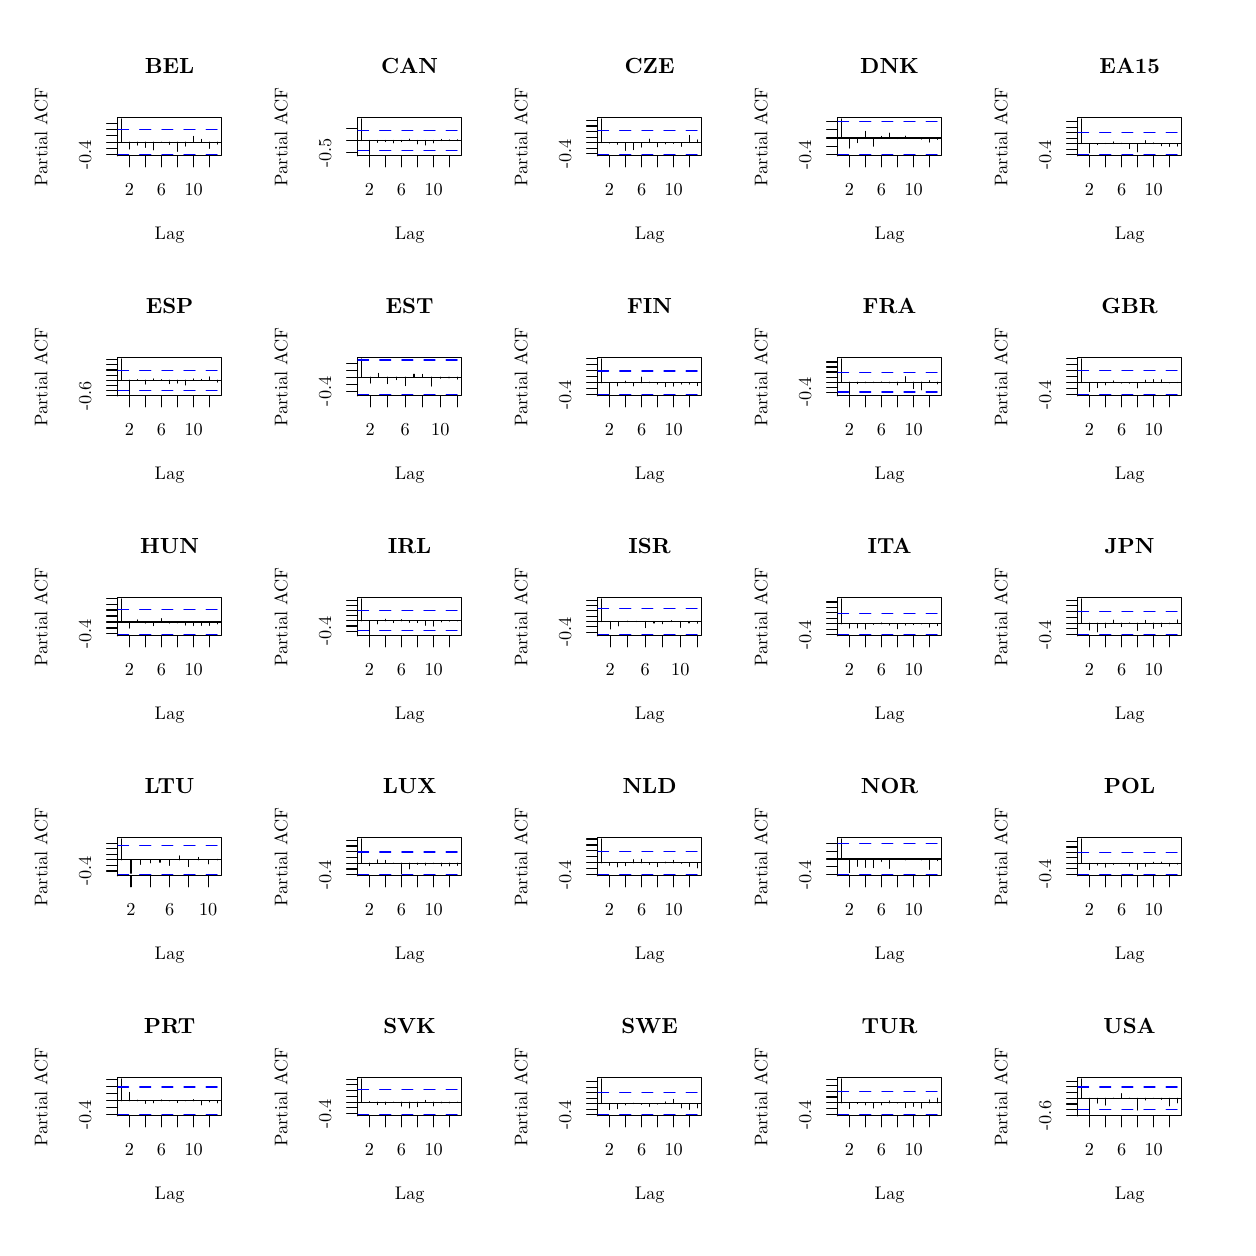
\begin{tikzpicture}[x=1pt,y=1pt]
\definecolor{fillColor}{RGB}{255,255,255}
\path[use as bounding box,fill=fillColor,fill opacity=0.00] (0,0) rectangle (433.62,433.62);
\begin{scope}
\path[clip] ( 32.47,387.29) rectangle ( 70.09,401.15);
\definecolor{drawColor}{RGB}{0,0,0}

\path[draw=drawColor,line width= 0.4pt,line join=round,line cap=round] ( 33.87,392.28) -- ( 33.87,400.63);

\path[draw=drawColor,line width= 0.4pt,line join=round,line cap=round] ( 36.77,392.28) -- ( 36.77,389.78);

\path[draw=drawColor,line width= 0.4pt,line join=round,line cap=round] ( 39.67,392.28) -- ( 39.67,391.21);

\path[draw=drawColor,line width= 0.4pt,line join=round,line cap=round] ( 42.57,392.28) -- ( 42.57,390.37);

\path[draw=drawColor,line width= 0.4pt,line join=round,line cap=round] ( 45.48,392.28) -- ( 45.48,389.48);

\path[draw=drawColor,line width= 0.4pt,line join=round,line cap=round] ( 48.38,392.28) -- ( 48.38,392.20);

\path[draw=drawColor,line width= 0.4pt,line join=round,line cap=round] ( 51.28,392.28) -- ( 51.28,391.47);

\path[draw=drawColor,line width= 0.4pt,line join=round,line cap=round] ( 54.18,392.28) -- ( 54.18,388.94);

\path[draw=drawColor,line width= 0.4pt,line join=round,line cap=round] ( 57.09,392.28) -- ( 57.09,390.83);

\path[draw=drawColor,line width= 0.4pt,line join=round,line cap=round] ( 59.99,392.28) -- ( 59.99,394.36);

\path[draw=drawColor,line width= 0.4pt,line join=round,line cap=round] ( 62.89,392.28) -- ( 62.89,393.21);

\path[draw=drawColor,line width= 0.4pt,line join=round,line cap=round] ( 65.80,392.28) -- ( 65.80,390.03);

\path[draw=drawColor,line width= 0.4pt,line join=round,line cap=round] ( 68.70,392.28) -- ( 68.70,391.52);
\end{scope}
\begin{scope}
\path[clip] (  0.00,  0.00) rectangle (433.62,433.62);
\definecolor{drawColor}{RGB}{0,0,0}

\path[draw=drawColor,line width= 0.4pt,line join=round,line cap=round] ( 36.77,387.29) -- ( 65.80,387.29);

\path[draw=drawColor,line width= 0.4pt,line join=round,line cap=round] ( 36.77,387.29) -- ( 36.77,383.33);

\path[draw=drawColor,line width= 0.4pt,line join=round,line cap=round] ( 42.57,387.29) -- ( 42.57,383.33);

\path[draw=drawColor,line width= 0.4pt,line join=round,line cap=round] ( 48.38,387.29) -- ( 48.38,383.33);

\path[draw=drawColor,line width= 0.4pt,line join=round,line cap=round] ( 54.18,387.29) -- ( 54.18,383.33);

\path[draw=drawColor,line width= 0.4pt,line join=round,line cap=round] ( 59.99,387.29) -- ( 59.99,383.33);

\path[draw=drawColor,line width= 0.4pt,line join=round,line cap=round] ( 65.80,387.29) -- ( 65.80,383.33);

\node[text=drawColor,anchor=base,inner sep=0pt, outer sep=0pt, scale=  0.66] at ( 36.77,373.03) {2};

\node[text=drawColor,anchor=base,inner sep=0pt, outer sep=0pt, scale=  0.66] at ( 48.38,373.03) {6};

\node[text=drawColor,anchor=base,inner sep=0pt, outer sep=0pt, scale=  0.66] at ( 59.99,373.03) {10};

\path[draw=drawColor,line width= 0.4pt,line join=round,line cap=round] ( 32.47,387.71) -- ( 32.47,399.13);

\path[draw=drawColor,line width= 0.4pt,line join=round,line cap=round] ( 32.47,387.71) -- ( 28.51,387.71);

\path[draw=drawColor,line width= 0.4pt,line join=round,line cap=round] ( 32.47,389.99) -- ( 28.51,389.99);

\path[draw=drawColor,line width= 0.4pt,line join=round,line cap=round] ( 32.47,392.28) -- ( 28.51,392.28);

\path[draw=drawColor,line width= 0.4pt,line join=round,line cap=round] ( 32.47,394.56) -- ( 28.51,394.56);

\path[draw=drawColor,line width= 0.4pt,line join=round,line cap=round] ( 32.47,396.85) -- ( 28.51,396.85);

\path[draw=drawColor,line width= 0.4pt,line join=round,line cap=round] ( 32.47,399.13) -- ( 28.51,399.13);

\node[text=drawColor,rotate= 90.00,anchor=base,inner sep=0pt, outer sep=0pt, scale=  0.66] at ( 22.97,387.71) {-0.4};

\path[draw=drawColor,line width= 0.4pt,line join=round,line cap=round] ( 32.47,387.29) --
	( 70.09,387.29) --
	( 70.09,401.15) --
	( 32.47,401.15) --
	( 32.47,387.29);
\end{scope}
\begin{scope}
\path[clip] (  0.00,346.90) rectangle ( 86.72,433.62);
\definecolor{drawColor}{RGB}{0,0,0}

\node[text=drawColor,anchor=base,inner sep=0pt, outer sep=0pt, scale=  0.66] at ( 51.28,357.19) {Lag};

\node[text=drawColor,rotate= 90.00,anchor=base,inner sep=0pt, outer sep=0pt, scale=  0.66] at (  7.13,394.22) {Partial ACF};
\end{scope}
\begin{scope}
\path[clip] ( 32.47,387.29) rectangle ( 70.09,401.15);
\definecolor{drawColor}{RGB}{0,0,0}

\path[draw=drawColor,line width= 0.4pt,line join=round,line cap=round] ( 32.47,392.28) -- ( 70.09,392.28);
\definecolor{drawColor}{RGB}{0,0,255}

\path[draw=drawColor,line width= 0.4pt,dash pattern=on 4pt off 4pt ,line join=round,line cap=round] ( 32.47,396.76) -- ( 70.09,396.76);

\path[draw=drawColor,line width= 0.4pt,dash pattern=on 4pt off 4pt ,line join=round,line cap=round] ( 32.47,387.80) -- ( 70.09,387.80);
\end{scope}
\begin{scope}
\path[clip] (  0.00,346.90) rectangle ( 86.72,433.62);
\definecolor{drawColor}{RGB}{0,0,0}

\node[text=drawColor,anchor=base,inner sep=0pt, outer sep=0pt, scale=  0.79] at ( 51.28,416.99) {\bfseries BEL};
\end{scope}
\begin{scope}
\path[clip] (119.20,387.29) rectangle (156.82,401.15);
\definecolor{drawColor}{RGB}{0,0,0}

\path[draw=drawColor,line width= 0.4pt,line join=round,line cap=round] (120.59,392.85) -- (120.59,400.63);

\path[draw=drawColor,line width= 0.4pt,line join=round,line cap=round] (123.49,392.85) -- (123.49,387.80);

\path[draw=drawColor,line width= 0.4pt,line join=round,line cap=round] (126.39,392.85) -- (126.39,392.15);

\path[draw=drawColor,line width= 0.4pt,line join=round,line cap=round] (129.30,392.85) -- (129.30,392.45);

\path[draw=drawColor,line width= 0.4pt,line join=round,line cap=round] (132.20,392.85) -- (132.20,391.97);

\path[draw=drawColor,line width= 0.4pt,line join=round,line cap=round] (135.10,392.85) -- (135.10,392.46);

\path[draw=drawColor,line width= 0.4pt,line join=round,line cap=round] (138.01,392.85) -- (138.01,393.33);

\path[draw=drawColor,line width= 0.4pt,line join=round,line cap=round] (140.91,392.85) -- (140.91,391.62);

\path[draw=drawColor,line width= 0.4pt,line join=round,line cap=round] (143.81,392.85) -- (143.81,391.23);

\path[draw=drawColor,line width= 0.4pt,line join=round,line cap=round] (146.71,392.85) -- (146.71,392.00);

\path[draw=drawColor,line width= 0.4pt,line join=round,line cap=round] (149.62,392.85) -- (149.62,393.22);

\path[draw=drawColor,line width= 0.4pt,line join=round,line cap=round] (152.52,392.85) -- (152.52,393.04);

\path[draw=drawColor,line width= 0.4pt,line join=round,line cap=round] (155.42,392.85) -- (155.42,393.10);
\end{scope}
\begin{scope}
\path[clip] (  0.00,  0.00) rectangle (433.62,433.62);
\definecolor{drawColor}{RGB}{0,0,0}

\path[draw=drawColor,line width= 0.4pt,line join=round,line cap=round] (123.49,387.29) -- (152.52,387.29);

\path[draw=drawColor,line width= 0.4pt,line join=round,line cap=round] (123.49,387.29) -- (123.49,383.33);

\path[draw=drawColor,line width= 0.4pt,line join=round,line cap=round] (129.30,387.29) -- (129.30,383.33);

\path[draw=drawColor,line width= 0.4pt,line join=round,line cap=round] (135.10,387.29) -- (135.10,383.33);

\path[draw=drawColor,line width= 0.4pt,line join=round,line cap=round] (140.91,387.29) -- (140.91,383.33);

\path[draw=drawColor,line width= 0.4pt,line join=round,line cap=round] (146.71,387.29) -- (146.71,383.33);

\path[draw=drawColor,line width= 0.4pt,line join=round,line cap=round] (152.52,387.29) -- (152.52,383.33);

\node[text=drawColor,anchor=base,inner sep=0pt, outer sep=0pt, scale=  0.66] at (123.49,373.03) {2};

\node[text=drawColor,anchor=base,inner sep=0pt, outer sep=0pt, scale=  0.66] at (135.10,373.03) {6};

\node[text=drawColor,anchor=base,inner sep=0pt, outer sep=0pt, scale=  0.66] at (146.71,373.03) {10};

\path[draw=drawColor,line width= 0.4pt,line join=round,line cap=round] (119.20,388.41) -- (119.20,397.28);

\path[draw=drawColor,line width= 0.4pt,line join=round,line cap=round] (119.20,388.41) -- (115.24,388.41);

\path[draw=drawColor,line width= 0.4pt,line join=round,line cap=round] (119.20,392.85) -- (115.24,392.85);

\path[draw=drawColor,line width= 0.4pt,line join=round,line cap=round] (119.20,397.28) -- (115.24,397.28);

\node[text=drawColor,rotate= 90.00,anchor=base,inner sep=0pt, outer sep=0pt, scale=  0.66] at (109.69,388.41) {-0.5};

\path[draw=drawColor,line width= 0.4pt,line join=round,line cap=round] (119.20,387.29) --
	(156.82,387.29) --
	(156.82,401.15) --
	(119.20,401.15) --
	(119.20,387.29);
\end{scope}
\begin{scope}
\path[clip] ( 86.72,346.90) rectangle (173.45,433.62);
\definecolor{drawColor}{RGB}{0,0,0}

\node[text=drawColor,anchor=base,inner sep=0pt, outer sep=0pt, scale=  0.66] at (138.01,357.19) {Lag};

\node[text=drawColor,rotate= 90.00,anchor=base,inner sep=0pt, outer sep=0pt, scale=  0.66] at ( 93.85,394.22) {Partial ACF};
\end{scope}
\begin{scope}
\path[clip] (119.20,387.29) rectangle (156.82,401.15);
\definecolor{drawColor}{RGB}{0,0,0}

\path[draw=drawColor,line width= 0.4pt,line join=round,line cap=round] (119.20,392.85) -- (156.82,392.85);
\definecolor{drawColor}{RGB}{0,0,255}

\path[draw=drawColor,line width= 0.4pt,dash pattern=on 4pt off 4pt ,line join=round,line cap=round] (119.20,396.32) -- (156.82,396.32);

\path[draw=drawColor,line width= 0.4pt,dash pattern=on 4pt off 4pt ,line join=round,line cap=round] (119.20,389.37) -- (156.82,389.37);
\end{scope}
\begin{scope}
\path[clip] ( 86.72,346.90) rectangle (173.45,433.62);
\definecolor{drawColor}{RGB}{0,0,0}

\node[text=drawColor,anchor=base,inner sep=0pt, outer sep=0pt, scale=  0.79] at (138.01,416.99) {\bfseries CAN};
\end{scope}
\begin{scope}
\path[clip] (205.92,387.29) rectangle (243.54,401.15);
\definecolor{drawColor}{RGB}{0,0,0}

\path[draw=drawColor,line width= 0.4pt,line join=round,line cap=round] (207.31,392.09) -- (207.31,400.63);

\path[draw=drawColor,line width= 0.4pt,line join=round,line cap=round] (210.22,392.09) -- (210.22,391.92);

\path[draw=drawColor,line width= 0.4pt,line join=round,line cap=round] (213.12,392.09) -- (213.12,391.50);

\path[draw=drawColor,line width= 0.4pt,line join=round,line cap=round] (216.02,392.09) -- (216.02,389.29);

\path[draw=drawColor,line width= 0.4pt,line join=round,line cap=round] (218.92,392.09) -- (218.92,389.57);

\path[draw=drawColor,line width= 0.4pt,line join=round,line cap=round] (221.83,392.09) -- (221.83,390.49);

\path[draw=drawColor,line width= 0.4pt,line join=round,line cap=round] (224.73,392.09) -- (224.73,393.30);

\path[draw=drawColor,line width= 0.4pt,line join=round,line cap=round] (227.63,392.09) -- (227.63,390.60);

\path[draw=drawColor,line width= 0.4pt,line join=round,line cap=round] (230.54,392.09) -- (230.54,391.67);

\path[draw=drawColor,line width= 0.4pt,line join=round,line cap=round] (233.44,392.09) -- (233.44,391.84);

\path[draw=drawColor,line width= 0.4pt,line join=round,line cap=round] (236.34,392.09) -- (236.34,390.71);

\path[draw=drawColor,line width= 0.4pt,line join=round,line cap=round] (239.24,392.09) -- (239.24,394.71);

\path[draw=drawColor,line width= 0.4pt,line join=round,line cap=round] (242.15,392.09) -- (242.15,393.03);
\end{scope}
\begin{scope}
\path[clip] (  0.00,  0.00) rectangle (433.62,433.62);
\definecolor{drawColor}{RGB}{0,0,0}

\path[draw=drawColor,line width= 0.4pt,line join=round,line cap=round] (210.22,387.29) -- (239.24,387.29);

\path[draw=drawColor,line width= 0.4pt,line join=round,line cap=round] (210.22,387.29) -- (210.22,383.33);

\path[draw=drawColor,line width= 0.4pt,line join=round,line cap=round] (216.02,387.29) -- (216.02,383.33);

\path[draw=drawColor,line width= 0.4pt,line join=round,line cap=round] (221.83,387.29) -- (221.83,383.33);

\path[draw=drawColor,line width= 0.4pt,line join=round,line cap=round] (227.63,387.29) -- (227.63,383.33);

\path[draw=drawColor,line width= 0.4pt,line join=round,line cap=round] (233.44,387.29) -- (233.44,383.33);

\path[draw=drawColor,line width= 0.4pt,line join=round,line cap=round] (239.24,387.29) -- (239.24,383.33);

\node[text=drawColor,anchor=base,inner sep=0pt, outer sep=0pt, scale=  0.66] at (210.22,373.03) {2};

\node[text=drawColor,anchor=base,inner sep=0pt, outer sep=0pt, scale=  0.66] at (221.83,373.03) {6};

\node[text=drawColor,anchor=base,inner sep=0pt, outer sep=0pt, scale=  0.66] at (233.44,373.03) {10};

\path[draw=drawColor,line width= 0.4pt,line join=round,line cap=round] (205.92,388.08) -- (205.92,400.10);

\path[draw=drawColor,line width= 0.4pt,line join=round,line cap=round] (205.92,388.08) -- (201.96,388.08);

\path[draw=drawColor,line width= 0.4pt,line join=round,line cap=round] (205.92,390.08) -- (201.96,390.08);

\path[draw=drawColor,line width= 0.4pt,line join=round,line cap=round] (205.92,392.09) -- (201.96,392.09);

\path[draw=drawColor,line width= 0.4pt,line join=round,line cap=round] (205.92,394.09) -- (201.96,394.09);

\path[draw=drawColor,line width= 0.4pt,line join=round,line cap=round] (205.92,396.10) -- (201.96,396.10);

\path[draw=drawColor,line width= 0.4pt,line join=round,line cap=round] (205.92,398.10) -- (201.96,398.10);

\path[draw=drawColor,line width= 0.4pt,line join=round,line cap=round] (205.92,400.10) -- (201.96,400.10);

\node[text=drawColor,rotate= 90.00,anchor=base,inner sep=0pt, outer sep=0pt, scale=  0.66] at (196.42,388.08) {-0.4};

\path[draw=drawColor,line width= 0.4pt,line join=round,line cap=round] (205.92,387.29) --
	(243.54,387.29) --
	(243.54,401.15) --
	(205.92,401.15) --
	(205.92,387.29);
\end{scope}
\begin{scope}
\path[clip] (173.45,346.90) rectangle (260.17,433.62);
\definecolor{drawColor}{RGB}{0,0,0}

\node[text=drawColor,anchor=base,inner sep=0pt, outer sep=0pt, scale=  0.66] at (224.73,357.19) {Lag};

\node[text=drawColor,rotate= 90.00,anchor=base,inner sep=0pt, outer sep=0pt, scale=  0.66] at (180.58,394.22) {Partial ACF};
\end{scope}
\begin{scope}
\path[clip] (205.92,387.29) rectangle (243.54,401.15);
\definecolor{drawColor}{RGB}{0,0,0}

\path[draw=drawColor,line width= 0.4pt,line join=round,line cap=round] (205.92,392.09) -- (243.54,392.09);
\definecolor{drawColor}{RGB}{0,0,255}

\path[draw=drawColor,line width= 0.4pt,dash pattern=on 4pt off 4pt ,line join=round,line cap=round] (205.92,396.37) -- (243.54,396.37);

\path[draw=drawColor,line width= 0.4pt,dash pattern=on 4pt off 4pt ,line join=round,line cap=round] (205.92,387.80) -- (243.54,387.80);
\end{scope}
\begin{scope}
\path[clip] (173.45,346.90) rectangle (260.17,433.62);
\definecolor{drawColor}{RGB}{0,0,0}

\node[text=drawColor,anchor=base,inner sep=0pt, outer sep=0pt, scale=  0.79] at (224.73,416.99) {\bfseries CZE};
\end{scope}
\begin{scope}
\path[clip] (292.64,387.29) rectangle (330.26,401.15);
\definecolor{drawColor}{RGB}{0,0,0}

\path[draw=drawColor,line width= 0.4pt,line join=round,line cap=round] (294.04,393.75) -- (294.04,400.63);

\path[draw=drawColor,line width= 0.4pt,line join=round,line cap=round] (296.94,393.75) -- (296.94,390.07);

\path[draw=drawColor,line width= 0.4pt,line join=round,line cap=round] (299.84,393.75) -- (299.84,392.11);

\path[draw=drawColor,line width= 0.4pt,line join=round,line cap=round] (302.75,393.75) -- (302.75,396.11);

\path[draw=drawColor,line width= 0.4pt,line join=round,line cap=round] (305.65,393.75) -- (305.65,390.78);

\path[draw=drawColor,line width= 0.4pt,line join=round,line cap=round] (308.55,393.75) -- (308.55,394.35);

\path[draw=drawColor,line width= 0.4pt,line join=round,line cap=round] (311.45,393.75) -- (311.45,395.47);

\path[draw=drawColor,line width= 0.4pt,line join=round,line cap=round] (314.36,393.75) -- (314.36,393.58);

\path[draw=drawColor,line width= 0.4pt,line join=round,line cap=round] (317.26,393.75) -- (317.26,394.43);

\path[draw=drawColor,line width= 0.4pt,line join=round,line cap=round] (320.16,393.75) -- (320.16,393.72);

\path[draw=drawColor,line width= 0.4pt,line join=round,line cap=round] (323.07,393.75) -- (323.07,393.33);

\path[draw=drawColor,line width= 0.4pt,line join=round,line cap=round] (325.97,393.75) -- (325.97,392.26);

\path[draw=drawColor,line width= 0.4pt,line join=round,line cap=round] (328.87,393.75) -- (328.87,393.27);
\end{scope}
\begin{scope}
\path[clip] (  0.00,  0.00) rectangle (433.62,433.62);
\definecolor{drawColor}{RGB}{0,0,0}

\path[draw=drawColor,line width= 0.4pt,line join=round,line cap=round] (296.94,387.29) -- (325.97,387.29);

\path[draw=drawColor,line width= 0.4pt,line join=round,line cap=round] (296.94,387.29) -- (296.94,383.33);

\path[draw=drawColor,line width= 0.4pt,line join=round,line cap=round] (302.75,387.29) -- (302.75,383.33);

\path[draw=drawColor,line width= 0.4pt,line join=round,line cap=round] (308.55,387.29) -- (308.55,383.33);

\path[draw=drawColor,line width= 0.4pt,line join=round,line cap=round] (314.36,387.29) -- (314.36,383.33);

\path[draw=drawColor,line width= 0.4pt,line join=round,line cap=round] (320.16,387.29) -- (320.16,383.33);

\path[draw=drawColor,line width= 0.4pt,line join=round,line cap=round] (325.97,387.29) -- (325.97,383.33);

\node[text=drawColor,anchor=base,inner sep=0pt, outer sep=0pt, scale=  0.66] at (296.94,373.03) {2};

\node[text=drawColor,anchor=base,inner sep=0pt, outer sep=0pt, scale=  0.66] at (308.55,373.03) {6};

\node[text=drawColor,anchor=base,inner sep=0pt, outer sep=0pt, scale=  0.66] at (320.16,373.03) {10};

\path[draw=drawColor,line width= 0.4pt,line join=round,line cap=round] (292.64,387.68) -- (292.64,399.82);

\path[draw=drawColor,line width= 0.4pt,line join=round,line cap=round] (292.64,387.68) -- (288.68,387.68);

\path[draw=drawColor,line width= 0.4pt,line join=round,line cap=round] (292.64,390.72) -- (288.68,390.72);

\path[draw=drawColor,line width= 0.4pt,line join=round,line cap=round] (292.64,393.75) -- (288.68,393.75);

\path[draw=drawColor,line width= 0.4pt,line join=round,line cap=round] (292.64,396.79) -- (288.68,396.79);

\path[draw=drawColor,line width= 0.4pt,line join=round,line cap=round] (292.64,399.82) -- (288.68,399.82);

\node[text=drawColor,rotate= 90.00,anchor=base,inner sep=0pt, outer sep=0pt, scale=  0.66] at (283.14,387.68) {-0.4};

\path[draw=drawColor,line width= 0.4pt,line join=round,line cap=round] (292.64,387.29) --
	(330.26,387.29) --
	(330.26,401.15) --
	(292.64,401.15) --
	(292.64,387.29);
\end{scope}
\begin{scope}
\path[clip] (260.17,346.90) rectangle (346.90,433.62);
\definecolor{drawColor}{RGB}{0,0,0}

\node[text=drawColor,anchor=base,inner sep=0pt, outer sep=0pt, scale=  0.66] at (311.45,357.19) {Lag};

\node[text=drawColor,rotate= 90.00,anchor=base,inner sep=0pt, outer sep=0pt, scale=  0.66] at (267.30,394.22) {Partial ACF};
\end{scope}
\begin{scope}
\path[clip] (292.64,387.29) rectangle (330.26,401.15);
\definecolor{drawColor}{RGB}{0,0,0}

\path[draw=drawColor,line width= 0.4pt,line join=round,line cap=round] (292.64,393.75) -- (330.26,393.75);
\definecolor{drawColor}{RGB}{0,0,255}

\path[draw=drawColor,line width= 0.4pt,dash pattern=on 4pt off 4pt ,line join=round,line cap=round] (292.64,399.70) -- (330.26,399.70);

\path[draw=drawColor,line width= 0.4pt,dash pattern=on 4pt off 4pt ,line join=round,line cap=round] (292.64,387.80) -- (330.26,387.80);
\end{scope}
\begin{scope}
\path[clip] (260.17,346.90) rectangle (346.90,433.62);
\definecolor{drawColor}{RGB}{0,0,0}

\node[text=drawColor,anchor=base,inner sep=0pt, outer sep=0pt, scale=  0.79] at (311.45,416.99) {\bfseries DNK};
\end{scope}
\begin{scope}
\path[clip] (379.37,387.29) rectangle (416.99,401.15);
\definecolor{drawColor}{RGB}{0,0,0}

\path[draw=drawColor,line width= 0.4pt,line join=round,line cap=round] (380.76,391.71) -- (380.76,400.63);

\path[draw=drawColor,line width= 0.4pt,line join=round,line cap=round] (383.66,391.71) -- (383.66,388.40);

\path[draw=drawColor,line width= 0.4pt,line join=round,line cap=round] (386.57,391.71) -- (386.57,391.36);

\path[draw=drawColor,line width= 0.4pt,line join=round,line cap=round] (389.47,391.71) -- (389.47,391.83);

\path[draw=drawColor,line width= 0.4pt,line join=round,line cap=round] (392.37,391.71) -- (392.37,392.30);

\path[draw=drawColor,line width= 0.4pt,line join=round,line cap=round] (395.28,391.71) -- (395.28,391.84);

\path[draw=drawColor,line width= 0.4pt,line join=round,line cap=round] (398.18,391.71) -- (398.18,389.91);

\path[draw=drawColor,line width= 0.4pt,line join=round,line cap=round] (401.08,391.71) -- (401.08,388.77);

\path[draw=drawColor,line width= 0.4pt,line join=round,line cap=round] (403.98,391.71) -- (403.98,392.76);

\path[draw=drawColor,line width= 0.4pt,line join=round,line cap=round] (406.89,391.71) -- (406.89,391.94);

\path[draw=drawColor,line width= 0.4pt,line join=round,line cap=round] (409.79,391.71) -- (409.79,390.96);

\path[draw=drawColor,line width= 0.4pt,line join=round,line cap=round] (412.69,391.71) -- (412.69,390.74);

\path[draw=drawColor,line width= 0.4pt,line join=round,line cap=round] (415.59,391.71) -- (415.59,390.85);
\end{scope}
\begin{scope}
\path[clip] (  0.00,  0.00) rectangle (433.62,433.62);
\definecolor{drawColor}{RGB}{0,0,0}

\path[draw=drawColor,line width= 0.4pt,line join=round,line cap=round] (383.66,387.29) -- (412.69,387.29);

\path[draw=drawColor,line width= 0.4pt,line join=round,line cap=round] (383.66,387.29) -- (383.66,383.33);

\path[draw=drawColor,line width= 0.4pt,line join=round,line cap=round] (389.47,387.29) -- (389.47,383.33);

\path[draw=drawColor,line width= 0.4pt,line join=round,line cap=round] (395.28,387.29) -- (395.28,383.33);

\path[draw=drawColor,line width= 0.4pt,line join=round,line cap=round] (401.08,387.29) -- (401.08,383.33);

\path[draw=drawColor,line width= 0.4pt,line join=round,line cap=round] (406.89,387.29) -- (406.89,383.33);

\path[draw=drawColor,line width= 0.4pt,line join=round,line cap=round] (412.69,387.29) -- (412.69,383.33);

\node[text=drawColor,anchor=base,inner sep=0pt, outer sep=0pt, scale=  0.66] at (383.66,373.03) {2};

\node[text=drawColor,anchor=base,inner sep=0pt, outer sep=0pt, scale=  0.66] at (395.28,373.03) {6};

\node[text=drawColor,anchor=base,inner sep=0pt, outer sep=0pt, scale=  0.66] at (406.89,373.03) {10};

\path[draw=drawColor,line width= 0.4pt,line join=round,line cap=round] (379.37,387.72) -- (379.37,399.67);

\path[draw=drawColor,line width= 0.4pt,line join=round,line cap=round] (379.37,387.72) -- (375.41,387.72);

\path[draw=drawColor,line width= 0.4pt,line join=round,line cap=round] (379.37,389.71) -- (375.41,389.71);

\path[draw=drawColor,line width= 0.4pt,line join=round,line cap=round] (379.37,391.71) -- (375.41,391.71);

\path[draw=drawColor,line width= 0.4pt,line join=round,line cap=round] (379.37,393.70) -- (375.41,393.70);

\path[draw=drawColor,line width= 0.4pt,line join=round,line cap=round] (379.37,395.69) -- (375.41,395.69);

\path[draw=drawColor,line width= 0.4pt,line join=round,line cap=round] (379.37,397.68) -- (375.41,397.68);

\path[draw=drawColor,line width= 0.4pt,line join=round,line cap=round] (379.37,399.67) -- (375.41,399.67);

\node[text=drawColor,rotate= 90.00,anchor=base,inner sep=0pt, outer sep=0pt, scale=  0.66] at (369.86,387.72) {-0.4};

\path[draw=drawColor,line width= 0.4pt,line join=round,line cap=round] (379.37,387.29) --
	(416.99,387.29) --
	(416.99,401.15) --
	(379.37,401.15) --
	(379.37,387.29);
\end{scope}
\begin{scope}
\path[clip] (346.90,346.90) rectangle (433.62,433.62);
\definecolor{drawColor}{RGB}{0,0,0}

\node[text=drawColor,anchor=base,inner sep=0pt, outer sep=0pt, scale=  0.66] at (398.18,357.19) {Lag};

\node[text=drawColor,rotate= 90.00,anchor=base,inner sep=0pt, outer sep=0pt, scale=  0.66] at (354.02,394.22) {Partial ACF};
\end{scope}
\begin{scope}
\path[clip] (379.37,387.29) rectangle (416.99,401.15);
\definecolor{drawColor}{RGB}{0,0,0}

\path[draw=drawColor,line width= 0.4pt,line join=round,line cap=round] (379.37,391.71) -- (416.99,391.71);
\definecolor{drawColor}{RGB}{0,0,255}

\path[draw=drawColor,line width= 0.4pt,dash pattern=on 4pt off 4pt ,line join=round,line cap=round] (379.37,395.61) -- (416.99,395.61);

\path[draw=drawColor,line width= 0.4pt,dash pattern=on 4pt off 4pt ,line join=round,line cap=round] (379.37,387.80) -- (416.99,387.80);
\end{scope}
\begin{scope}
\path[clip] (346.90,346.90) rectangle (433.62,433.62);
\definecolor{drawColor}{RGB}{0,0,0}

\node[text=drawColor,anchor=base,inner sep=0pt, outer sep=0pt, scale=  0.79] at (398.18,416.99) {\bfseries EA15};
\end{scope}
\begin{scope}
\path[clip] ( 32.47,300.56) rectangle ( 70.09,314.42);
\definecolor{drawColor}{RGB}{0,0,0}

\path[draw=drawColor,line width= 0.4pt,line join=round,line cap=round] ( 33.87,306.21) -- ( 33.87,313.91);

\path[draw=drawColor,line width= 0.4pt,line join=round,line cap=round] ( 36.77,306.21) -- ( 36.77,301.08);

\path[draw=drawColor,line width= 0.4pt,line join=round,line cap=round] ( 39.67,306.21) -- ( 39.67,306.44);

\path[draw=drawColor,line width= 0.4pt,line join=round,line cap=round] ( 42.57,306.21) -- ( 42.57,304.81);

\path[draw=drawColor,line width= 0.4pt,line join=round,line cap=round] ( 45.48,306.21) -- ( 45.48,306.73);

\path[draw=drawColor,line width= 0.4pt,line join=round,line cap=round] ( 48.38,306.21) -- ( 48.38,306.46);

\path[draw=drawColor,line width= 0.4pt,line join=round,line cap=round] ( 51.28,306.21) -- ( 51.28,305.02);

\path[draw=drawColor,line width= 0.4pt,line join=round,line cap=round] ( 54.18,306.21) -- ( 54.18,305.17);

\path[draw=drawColor,line width= 0.4pt,line join=round,line cap=round] ( 57.09,306.21) -- ( 57.09,304.51);

\path[draw=drawColor,line width= 0.4pt,line join=round,line cap=round] ( 59.99,306.21) -- ( 59.99,306.71);

\path[draw=drawColor,line width= 0.4pt,line join=round,line cap=round] ( 62.89,306.21) -- ( 62.89,306.52);

\path[draw=drawColor,line width= 0.4pt,line join=round,line cap=round] ( 65.80,306.21) -- ( 65.80,307.45);

\path[draw=drawColor,line width= 0.4pt,line join=round,line cap=round] ( 68.70,306.21) -- ( 68.70,305.51);
\end{scope}
\begin{scope}
\path[clip] (  0.00,  0.00) rectangle (433.62,433.62);
\definecolor{drawColor}{RGB}{0,0,0}

\path[draw=drawColor,line width= 0.4pt,line join=round,line cap=round] ( 36.77,300.56) -- ( 65.80,300.56);

\path[draw=drawColor,line width= 0.4pt,line join=round,line cap=round] ( 36.77,300.56) -- ( 36.77,296.60);

\path[draw=drawColor,line width= 0.4pt,line join=round,line cap=round] ( 42.57,300.56) -- ( 42.57,296.60);

\path[draw=drawColor,line width= 0.4pt,line join=round,line cap=round] ( 48.38,300.56) -- ( 48.38,296.60);

\path[draw=drawColor,line width= 0.4pt,line join=round,line cap=round] ( 54.18,300.56) -- ( 54.18,296.60);

\path[draw=drawColor,line width= 0.4pt,line join=round,line cap=round] ( 59.99,300.56) -- ( 59.99,296.60);

\path[draw=drawColor,line width= 0.4pt,line join=round,line cap=round] ( 65.80,300.56) -- ( 65.80,296.60);

\node[text=drawColor,anchor=base,inner sep=0pt, outer sep=0pt, scale=  0.66] at ( 36.77,286.31) {2};

\node[text=drawColor,anchor=base,inner sep=0pt, outer sep=0pt, scale=  0.66] at ( 48.38,286.31) {6};

\node[text=drawColor,anchor=base,inner sep=0pt, outer sep=0pt, scale=  0.66] at ( 59.99,286.31) {10};

\path[draw=drawColor,line width= 0.4pt,line join=round,line cap=round] ( 32.47,300.64) -- ( 32.47,313.64);

\path[draw=drawColor,line width= 0.4pt,line join=round,line cap=round] ( 32.47,300.64) -- ( 28.51,300.64);

\path[draw=drawColor,line width= 0.4pt,line join=round,line cap=round] ( 32.47,302.49) -- ( 28.51,302.49);

\path[draw=drawColor,line width= 0.4pt,line join=round,line cap=round] ( 32.47,304.35) -- ( 28.51,304.35);

\path[draw=drawColor,line width= 0.4pt,line join=round,line cap=round] ( 32.47,306.21) -- ( 28.51,306.21);

\path[draw=drawColor,line width= 0.4pt,line join=round,line cap=round] ( 32.47,308.07) -- ( 28.51,308.07);

\path[draw=drawColor,line width= 0.4pt,line join=round,line cap=round] ( 32.47,309.93) -- ( 28.51,309.93);

\path[draw=drawColor,line width= 0.4pt,line join=round,line cap=round] ( 32.47,311.79) -- ( 28.51,311.79);

\path[draw=drawColor,line width= 0.4pt,line join=round,line cap=round] ( 32.47,313.64) -- ( 28.51,313.64);

\node[text=drawColor,rotate= 90.00,anchor=base,inner sep=0pt, outer sep=0pt, scale=  0.66] at ( 22.97,300.64) {-0.6};

\path[draw=drawColor,line width= 0.4pt,line join=round,line cap=round] ( 32.47,300.56) --
	( 70.09,300.56) --
	( 70.09,314.42) --
	( 32.47,314.42) --
	( 32.47,300.56);
\end{scope}
\begin{scope}
\path[clip] (  0.00,260.17) rectangle ( 86.72,346.90);
\definecolor{drawColor}{RGB}{0,0,0}

\node[text=drawColor,anchor=base,inner sep=0pt, outer sep=0pt, scale=  0.66] at ( 51.28,270.47) {Lag};

\node[text=drawColor,rotate= 90.00,anchor=base,inner sep=0pt, outer sep=0pt, scale=  0.66] at (  7.13,307.49) {Partial ACF};
\end{scope}
\begin{scope}
\path[clip] ( 32.47,300.56) rectangle ( 70.09,314.42);
\definecolor{drawColor}{RGB}{0,0,0}

\path[draw=drawColor,line width= 0.4pt,line join=round,line cap=round] ( 32.47,306.21) -- ( 70.09,306.21);
\definecolor{drawColor}{RGB}{0,0,255}

\path[draw=drawColor,line width= 0.4pt,dash pattern=on 4pt off 4pt ,line join=round,line cap=round] ( 32.47,309.85) -- ( 70.09,309.85);

\path[draw=drawColor,line width= 0.4pt,dash pattern=on 4pt off 4pt ,line join=round,line cap=round] ( 32.47,302.57) -- ( 70.09,302.57);
\end{scope}
\begin{scope}
\path[clip] (  0.00,260.17) rectangle ( 86.72,346.90);
\definecolor{drawColor}{RGB}{0,0,0}

\node[text=drawColor,anchor=base,inner sep=0pt, outer sep=0pt, scale=  0.79] at ( 51.28,330.26) {\bfseries ESP};
\end{scope}
\begin{scope}
\path[clip] (119.20,300.56) rectangle (156.82,314.42);
\definecolor{drawColor}{RGB}{0,0,0}

\path[draw=drawColor,line width= 0.4pt,line join=round,line cap=round] (120.59,307.31) -- (120.59,313.91);

\path[draw=drawColor,line width= 0.4pt,line join=round,line cap=round] (123.76,307.31) -- (123.76,305.19);

\path[draw=drawColor,line width= 0.4pt,line join=round,line cap=round] (126.92,307.31) -- (126.92,308.69);

\path[draw=drawColor,line width= 0.4pt,line join=round,line cap=round] (130.09,307.31) -- (130.09,305.00);

\path[draw=drawColor,line width= 0.4pt,line join=round,line cap=round] (133.26,307.31) -- (133.26,306.44);

\path[draw=drawColor,line width= 0.4pt,line join=round,line cap=round] (136.42,307.31) -- (136.42,304.30);

\path[draw=drawColor,line width= 0.4pt,line join=round,line cap=round] (139.59,307.31) -- (139.59,308.41);

\path[draw=drawColor,line width= 0.4pt,line join=round,line cap=round] (142.76,307.31) -- (142.76,308.33);

\path[draw=drawColor,line width= 0.4pt,line join=round,line cap=round] (145.92,307.31) -- (145.92,304.12);

\path[draw=drawColor,line width= 0.4pt,line join=round,line cap=round] (149.09,307.31) -- (149.09,306.95);

\path[draw=drawColor,line width= 0.4pt,line join=round,line cap=round] (152.26,307.31) -- (152.26,307.11);

\path[draw=drawColor,line width= 0.4pt,line join=round,line cap=round] (155.42,307.31) -- (155.42,306.63);
\end{scope}
\begin{scope}
\path[clip] (  0.00,  0.00) rectangle (433.62,433.62);
\definecolor{drawColor}{RGB}{0,0,0}

\path[draw=drawColor,line width= 0.4pt,line join=round,line cap=round] (123.76,300.56) -- (155.42,300.56);

\path[draw=drawColor,line width= 0.4pt,line join=round,line cap=round] (123.76,300.56) -- (123.76,296.60);

\path[draw=drawColor,line width= 0.4pt,line join=round,line cap=round] (130.09,300.56) -- (130.09,296.60);

\path[draw=drawColor,line width= 0.4pt,line join=round,line cap=round] (136.42,300.56) -- (136.42,296.60);

\path[draw=drawColor,line width= 0.4pt,line join=round,line cap=round] (142.76,300.56) -- (142.76,296.60);

\path[draw=drawColor,line width= 0.4pt,line join=round,line cap=round] (149.09,300.56) -- (149.09,296.60);

\path[draw=drawColor,line width= 0.4pt,line join=round,line cap=round] (155.42,300.56) -- (155.42,296.60);

\node[text=drawColor,anchor=base,inner sep=0pt, outer sep=0pt, scale=  0.66] at (123.76,286.31) {2};

\node[text=drawColor,anchor=base,inner sep=0pt, outer sep=0pt, scale=  0.66] at (136.42,286.31) {6};

\node[text=drawColor,anchor=base,inner sep=0pt, outer sep=0pt, scale=  0.66] at (149.09,286.31) {10};

\path[draw=drawColor,line width= 0.4pt,line join=round,line cap=round] (119.20,302.22) -- (119.20,312.39);

\path[draw=drawColor,line width= 0.4pt,line join=round,line cap=round] (119.20,302.22) -- (115.24,302.22);

\path[draw=drawColor,line width= 0.4pt,line join=round,line cap=round] (119.20,304.76) -- (115.24,304.76);

\path[draw=drawColor,line width= 0.4pt,line join=round,line cap=round] (119.20,307.31) -- (115.24,307.31);

\path[draw=drawColor,line width= 0.4pt,line join=round,line cap=round] (119.20,309.85) -- (115.24,309.85);

\path[draw=drawColor,line width= 0.4pt,line join=round,line cap=round] (119.20,312.39) -- (115.24,312.39);

\node[text=drawColor,rotate= 90.00,anchor=base,inner sep=0pt, outer sep=0pt, scale=  0.66] at (109.69,302.22) {-0.4};

\path[draw=drawColor,line width= 0.4pt,line join=round,line cap=round] (119.20,300.56) --
	(156.82,300.56) --
	(156.82,314.42) --
	(119.20,314.42) --
	(119.20,300.56);
\end{scope}
\begin{scope}
\path[clip] ( 86.72,260.17) rectangle (173.45,346.90);
\definecolor{drawColor}{RGB}{0,0,0}

\node[text=drawColor,anchor=base,inner sep=0pt, outer sep=0pt, scale=  0.66] at (138.01,270.47) {Lag};

\node[text=drawColor,rotate= 90.00,anchor=base,inner sep=0pt, outer sep=0pt, scale=  0.66] at ( 93.85,307.49) {Partial ACF};
\end{scope}
\begin{scope}
\path[clip] (119.20,300.56) rectangle (156.82,314.42);
\definecolor{drawColor}{RGB}{0,0,0}

\path[draw=drawColor,line width= 0.4pt,line join=round,line cap=round] (119.20,307.31) -- (156.82,307.31);
\definecolor{drawColor}{RGB}{0,0,255}

\path[draw=drawColor,line width= 0.4pt,dash pattern=on 4pt off 4pt ,line join=round,line cap=round] (119.20,313.54) -- (156.82,313.54);

\path[draw=drawColor,line width= 0.4pt,dash pattern=on 4pt off 4pt ,line join=round,line cap=round] (119.20,301.08) -- (156.82,301.08);
\end{scope}
\begin{scope}
\path[clip] ( 86.72,260.17) rectangle (173.45,346.90);
\definecolor{drawColor}{RGB}{0,0,0}

\node[text=drawColor,anchor=base,inner sep=0pt, outer sep=0pt, scale=  0.79] at (138.01,330.26) {\bfseries EST};
\end{scope}
\begin{scope}
\path[clip] (205.92,300.56) rectangle (243.54,314.42);
\definecolor{drawColor}{RGB}{0,0,0}

\path[draw=drawColor,line width= 0.4pt,line join=round,line cap=round] (207.31,305.32) -- (207.31,313.91);

\path[draw=drawColor,line width= 0.4pt,line join=round,line cap=round] (210.22,305.32) -- (210.22,301.14);

\path[draw=drawColor,line width= 0.4pt,line join=round,line cap=round] (213.12,305.32) -- (213.12,304.16);

\path[draw=drawColor,line width= 0.4pt,line join=round,line cap=round] (216.02,305.32) -- (216.02,305.85);

\path[draw=drawColor,line width= 0.4pt,line join=round,line cap=round] (218.92,305.32) -- (218.92,304.16);

\path[draw=drawColor,line width= 0.4pt,line join=round,line cap=round] (221.83,305.32) -- (221.83,307.34);

\path[draw=drawColor,line width= 0.4pt,line join=round,line cap=round] (224.73,305.32) -- (224.73,305.50);

\path[draw=drawColor,line width= 0.4pt,line join=round,line cap=round] (227.63,305.32) -- (227.63,304.84);

\path[draw=drawColor,line width= 0.4pt,line join=round,line cap=round] (230.54,305.32) -- (230.54,303.89);

\path[draw=drawColor,line width= 0.4pt,line join=round,line cap=round] (233.44,305.32) -- (233.44,304.10);

\path[draw=drawColor,line width= 0.4pt,line join=round,line cap=round] (236.34,305.32) -- (236.34,304.80);

\path[draw=drawColor,line width= 0.4pt,line join=round,line cap=round] (239.24,305.32) -- (239.24,304.80);

\path[draw=drawColor,line width= 0.4pt,line join=round,line cap=round] (242.15,305.32) -- (242.15,304.28);
\end{scope}
\begin{scope}
\path[clip] (  0.00,  0.00) rectangle (433.62,433.62);
\definecolor{drawColor}{RGB}{0,0,0}

\path[draw=drawColor,line width= 0.4pt,line join=round,line cap=round] (210.22,300.56) -- (239.24,300.56);

\path[draw=drawColor,line width= 0.4pt,line join=round,line cap=round] (210.22,300.56) -- (210.22,296.60);

\path[draw=drawColor,line width= 0.4pt,line join=round,line cap=round] (216.02,300.56) -- (216.02,296.60);

\path[draw=drawColor,line width= 0.4pt,line join=round,line cap=round] (221.83,300.56) -- (221.83,296.60);

\path[draw=drawColor,line width= 0.4pt,line join=round,line cap=round] (227.63,300.56) -- (227.63,296.60);

\path[draw=drawColor,line width= 0.4pt,line join=round,line cap=round] (233.44,300.56) -- (233.44,296.60);

\path[draw=drawColor,line width= 0.4pt,line join=round,line cap=round] (239.24,300.56) -- (239.24,296.60);

\node[text=drawColor,anchor=base,inner sep=0pt, outer sep=0pt, scale=  0.66] at (210.22,286.31) {2};

\node[text=drawColor,anchor=base,inner sep=0pt, outer sep=0pt, scale=  0.66] at (221.83,286.31) {6};

\node[text=drawColor,anchor=base,inner sep=0pt, outer sep=0pt, scale=  0.66] at (233.44,286.31) {10};

\path[draw=drawColor,line width= 0.4pt,line join=round,line cap=round] (205.92,300.99) -- (205.92,313.97);

\path[draw=drawColor,line width= 0.4pt,line join=round,line cap=round] (205.92,300.99) -- (201.96,300.99);

\path[draw=drawColor,line width= 0.4pt,line join=round,line cap=round] (205.92,303.15) -- (201.96,303.15);

\path[draw=drawColor,line width= 0.4pt,line join=round,line cap=round] (205.92,305.32) -- (201.96,305.32);

\path[draw=drawColor,line width= 0.4pt,line join=round,line cap=round] (205.92,307.48) -- (201.96,307.48);

\path[draw=drawColor,line width= 0.4pt,line join=round,line cap=round] (205.92,309.64) -- (201.96,309.64);

\path[draw=drawColor,line width= 0.4pt,line join=round,line cap=round] (205.92,311.80) -- (201.96,311.80);

\path[draw=drawColor,line width= 0.4pt,line join=round,line cap=round] (205.92,313.97) -- (201.96,313.97);

\node[text=drawColor,rotate= 90.00,anchor=base,inner sep=0pt, outer sep=0pt, scale=  0.66] at (196.42,300.99) {-0.4};

\path[draw=drawColor,line width= 0.4pt,line join=round,line cap=round] (205.92,300.56) --
	(243.54,300.56) --
	(243.54,314.42) --
	(205.92,314.42) --
	(205.92,300.56);
\end{scope}
\begin{scope}
\path[clip] (173.45,260.17) rectangle (260.17,346.90);
\definecolor{drawColor}{RGB}{0,0,0}

\node[text=drawColor,anchor=base,inner sep=0pt, outer sep=0pt, scale=  0.66] at (224.73,270.47) {Lag};

\node[text=drawColor,rotate= 90.00,anchor=base,inner sep=0pt, outer sep=0pt, scale=  0.66] at (180.58,307.49) {Partial ACF};
\end{scope}
\begin{scope}
\path[clip] (205.92,300.56) rectangle (243.54,314.42);
\definecolor{drawColor}{RGB}{0,0,0}

\path[draw=drawColor,line width= 0.4pt,line join=round,line cap=round] (205.92,305.32) -- (243.54,305.32);
\definecolor{drawColor}{RGB}{0,0,255}

\path[draw=drawColor,line width= 0.4pt,dash pattern=on 4pt off 4pt ,line join=round,line cap=round] (205.92,309.55) -- (243.54,309.55);

\path[draw=drawColor,line width= 0.4pt,dash pattern=on 4pt off 4pt ,line join=round,line cap=round] (205.92,301.08) -- (243.54,301.08);
\end{scope}
\begin{scope}
\path[clip] (173.45,260.17) rectangle (260.17,346.90);
\definecolor{drawColor}{RGB}{0,0,0}

\node[text=drawColor,anchor=base,inner sep=0pt, outer sep=0pt, scale=  0.79] at (224.73,330.26) {\bfseries FIN};
\end{scope}
\begin{scope}
\path[clip] (292.64,300.56) rectangle (330.26,314.42);
\definecolor{drawColor}{RGB}{0,0,0}

\path[draw=drawColor,line width= 0.4pt,line join=round,line cap=round] (294.04,305.54) -- (294.04,313.91);

\path[draw=drawColor,line width= 0.4pt,line join=round,line cap=round] (296.94,305.54) -- (296.94,301.08);

\path[draw=drawColor,line width= 0.4pt,line join=round,line cap=round] (299.84,305.54) -- (299.84,305.02);

\path[draw=drawColor,line width= 0.4pt,line join=round,line cap=round] (302.75,305.54) -- (302.75,305.32);

\path[draw=drawColor,line width= 0.4pt,line join=round,line cap=round] (305.65,305.54) -- (305.65,305.40);

\path[draw=drawColor,line width= 0.4pt,line join=round,line cap=round] (308.55,305.54) -- (308.55,305.59);

\path[draw=drawColor,line width= 0.4pt,line join=round,line cap=round] (311.45,305.54) -- (311.45,305.30);

\path[draw=drawColor,line width= 0.4pt,line join=round,line cap=round] (314.36,305.54) -- (314.36,304.54);

\path[draw=drawColor,line width= 0.4pt,line join=round,line cap=round] (317.26,305.54) -- (317.26,307.48);

\path[draw=drawColor,line width= 0.4pt,line join=round,line cap=round] (320.16,305.54) -- (320.16,303.18);

\path[draw=drawColor,line width= 0.4pt,line join=round,line cap=round] (323.07,305.54) -- (323.07,302.72);

\path[draw=drawColor,line width= 0.4pt,line join=round,line cap=round] (325.97,305.54) -- (325.97,306.10);

\path[draw=drawColor,line width= 0.4pt,line join=round,line cap=round] (328.87,305.54) -- (328.87,304.88);
\end{scope}
\begin{scope}
\path[clip] (  0.00,  0.00) rectangle (433.62,433.62);
\definecolor{drawColor}{RGB}{0,0,0}

\path[draw=drawColor,line width= 0.4pt,line join=round,line cap=round] (296.94,300.56) -- (325.97,300.56);

\path[draw=drawColor,line width= 0.4pt,line join=round,line cap=round] (296.94,300.56) -- (296.94,296.60);

\path[draw=drawColor,line width= 0.4pt,line join=round,line cap=round] (302.75,300.56) -- (302.75,296.60);

\path[draw=drawColor,line width= 0.4pt,line join=round,line cap=round] (308.55,300.56) -- (308.55,296.60);

\path[draw=drawColor,line width= 0.4pt,line join=round,line cap=round] (314.36,300.56) -- (314.36,296.60);

\path[draw=drawColor,line width= 0.4pt,line join=round,line cap=round] (320.16,300.56) -- (320.16,296.60);

\path[draw=drawColor,line width= 0.4pt,line join=round,line cap=round] (325.97,300.56) -- (325.97,296.60);

\node[text=drawColor,anchor=base,inner sep=0pt, outer sep=0pt, scale=  0.66] at (296.94,286.31) {2};

\node[text=drawColor,anchor=base,inner sep=0pt, outer sep=0pt, scale=  0.66] at (308.55,286.31) {6};

\node[text=drawColor,anchor=base,inner sep=0pt, outer sep=0pt, scale=  0.66] at (320.16,286.31) {10};

\path[draw=drawColor,line width= 0.4pt,line join=round,line cap=round] (292.64,301.89) -- (292.64,312.82);

\path[draw=drawColor,line width= 0.4pt,line join=round,line cap=round] (292.64,301.89) -- (288.68,301.89);

\path[draw=drawColor,line width= 0.4pt,line join=round,line cap=round] (292.64,303.71) -- (288.68,303.71);

\path[draw=drawColor,line width= 0.4pt,line join=round,line cap=round] (292.64,305.54) -- (288.68,305.54);

\path[draw=drawColor,line width= 0.4pt,line join=round,line cap=round] (292.64,307.36) -- (288.68,307.36);

\path[draw=drawColor,line width= 0.4pt,line join=round,line cap=round] (292.64,309.18) -- (288.68,309.18);

\path[draw=drawColor,line width= 0.4pt,line join=round,line cap=round] (292.64,311.00) -- (288.68,311.00);

\path[draw=drawColor,line width= 0.4pt,line join=round,line cap=round] (292.64,312.82) -- (288.68,312.82);

\node[text=drawColor,rotate= 90.00,anchor=base,inner sep=0pt, outer sep=0pt, scale=  0.66] at (283.14,301.89) {-0.4};

\path[draw=drawColor,line width= 0.4pt,line join=round,line cap=round] (292.64,300.56) --
	(330.26,300.56) --
	(330.26,314.42) --
	(292.64,314.42) --
	(292.64,300.56);
\end{scope}
\begin{scope}
\path[clip] (260.17,260.17) rectangle (346.90,346.90);
\definecolor{drawColor}{RGB}{0,0,0}

\node[text=drawColor,anchor=base,inner sep=0pt, outer sep=0pt, scale=  0.66] at (311.45,270.47) {Lag};

\node[text=drawColor,rotate= 90.00,anchor=base,inner sep=0pt, outer sep=0pt, scale=  0.66] at (267.30,307.49) {Partial ACF};
\end{scope}
\begin{scope}
\path[clip] (292.64,300.56) rectangle (330.26,314.42);
\definecolor{drawColor}{RGB}{0,0,0}

\path[draw=drawColor,line width= 0.4pt,line join=round,line cap=round] (292.64,305.54) -- (330.26,305.54);
\definecolor{drawColor}{RGB}{0,0,255}

\path[draw=drawColor,line width= 0.4pt,dash pattern=on 4pt off 4pt ,line join=round,line cap=round] (292.64,309.11) -- (330.26,309.11);

\path[draw=drawColor,line width= 0.4pt,dash pattern=on 4pt off 4pt ,line join=round,line cap=round] (292.64,301.97) -- (330.26,301.97);
\end{scope}
\begin{scope}
\path[clip] (260.17,260.17) rectangle (346.90,346.90);
\definecolor{drawColor}{RGB}{0,0,0}

\node[text=drawColor,anchor=base,inner sep=0pt, outer sep=0pt, scale=  0.79] at (311.45,330.26) {\bfseries FRA};
\end{scope}
\begin{scope}
\path[clip] (379.37,300.56) rectangle (416.99,314.42);
\definecolor{drawColor}{RGB}{0,0,0}

\path[draw=drawColor,line width= 0.4pt,line join=round,line cap=round] (380.76,305.38) -- (380.76,313.91);

\path[draw=drawColor,line width= 0.4pt,line join=round,line cap=round] (383.66,305.38) -- (383.66,302.08);

\path[draw=drawColor,line width= 0.4pt,line join=round,line cap=round] (386.57,305.38) -- (386.57,303.55);

\path[draw=drawColor,line width= 0.4pt,line join=round,line cap=round] (389.47,305.38) -- (389.47,304.56);

\path[draw=drawColor,line width= 0.4pt,line join=round,line cap=round] (392.37,305.38) -- (392.37,306.01);

\path[draw=drawColor,line width= 0.4pt,line join=round,line cap=round] (395.28,305.38) -- (395.28,305.19);

\path[draw=drawColor,line width= 0.4pt,line join=round,line cap=round] (398.18,305.38) -- (398.18,305.14);

\path[draw=drawColor,line width= 0.4pt,line join=round,line cap=round] (401.08,305.38) -- (401.08,303.47);

\path[draw=drawColor,line width= 0.4pt,line join=round,line cap=round] (403.98,305.38) -- (403.98,306.28);

\path[draw=drawColor,line width= 0.4pt,line join=round,line cap=round] (406.89,305.38) -- (406.89,306.42);

\path[draw=drawColor,line width= 0.4pt,line join=round,line cap=round] (409.79,305.38) -- (409.79,306.38);

\path[draw=drawColor,line width= 0.4pt,line join=round,line cap=round] (412.69,305.38) -- (412.69,305.29);

\path[draw=drawColor,line width= 0.4pt,line join=round,line cap=round] (415.59,305.38) -- (415.59,305.42);
\end{scope}
\begin{scope}
\path[clip] (  0.00,  0.00) rectangle (433.62,433.62);
\definecolor{drawColor}{RGB}{0,0,0}

\path[draw=drawColor,line width= 0.4pt,line join=round,line cap=round] (383.66,300.56) -- (412.69,300.56);

\path[draw=drawColor,line width= 0.4pt,line join=round,line cap=round] (383.66,300.56) -- (383.66,296.60);

\path[draw=drawColor,line width= 0.4pt,line join=round,line cap=round] (389.47,300.56) -- (389.47,296.60);

\path[draw=drawColor,line width= 0.4pt,line join=round,line cap=round] (395.28,300.56) -- (395.28,296.60);

\path[draw=drawColor,line width= 0.4pt,line join=round,line cap=round] (401.08,300.56) -- (401.08,296.60);

\path[draw=drawColor,line width= 0.4pt,line join=round,line cap=round] (406.89,300.56) -- (406.89,296.60);

\path[draw=drawColor,line width= 0.4pt,line join=round,line cap=round] (412.69,300.56) -- (412.69,296.60);

\node[text=drawColor,anchor=base,inner sep=0pt, outer sep=0pt, scale=  0.66] at (383.66,286.31) {2};

\node[text=drawColor,anchor=base,inner sep=0pt, outer sep=0pt, scale=  0.66] at (395.28,286.31) {6};

\node[text=drawColor,anchor=base,inner sep=0pt, outer sep=0pt, scale=  0.66] at (406.89,286.31) {10};

\path[draw=drawColor,line width= 0.4pt,line join=round,line cap=round] (379.37,300.99) -- (379.37,314.16);

\path[draw=drawColor,line width= 0.4pt,line join=round,line cap=round] (379.37,300.99) -- (375.41,300.99);

\path[draw=drawColor,line width= 0.4pt,line join=round,line cap=round] (379.37,303.19) -- (375.41,303.19);

\path[draw=drawColor,line width= 0.4pt,line join=round,line cap=round] (379.37,305.38) -- (375.41,305.38);

\path[draw=drawColor,line width= 0.4pt,line join=round,line cap=round] (379.37,307.58) -- (375.41,307.58);

\path[draw=drawColor,line width= 0.4pt,line join=round,line cap=round] (379.37,309.77) -- (375.41,309.77);

\path[draw=drawColor,line width= 0.4pt,line join=round,line cap=round] (379.37,311.97) -- (375.41,311.97);

\path[draw=drawColor,line width= 0.4pt,line join=round,line cap=round] (379.37,314.16) -- (375.41,314.16);

\node[text=drawColor,rotate= 90.00,anchor=base,inner sep=0pt, outer sep=0pt, scale=  0.66] at (369.86,300.99) {-0.4};

\path[draw=drawColor,line width= 0.4pt,line join=round,line cap=round] (379.37,300.56) --
	(416.99,300.56) --
	(416.99,314.42) --
	(379.37,314.42) --
	(379.37,300.56);
\end{scope}
\begin{scope}
\path[clip] (346.90,260.17) rectangle (433.62,346.90);
\definecolor{drawColor}{RGB}{0,0,0}

\node[text=drawColor,anchor=base,inner sep=0pt, outer sep=0pt, scale=  0.66] at (398.18,270.47) {Lag};

\node[text=drawColor,rotate= 90.00,anchor=base,inner sep=0pt, outer sep=0pt, scale=  0.66] at (354.02,307.49) {Partial ACF};
\end{scope}
\begin{scope}
\path[clip] (379.37,300.56) rectangle (416.99,314.42);
\definecolor{drawColor}{RGB}{0,0,0}

\path[draw=drawColor,line width= 0.4pt,line join=round,line cap=round] (379.37,305.38) -- (416.99,305.38);
\definecolor{drawColor}{RGB}{0,0,255}

\path[draw=drawColor,line width= 0.4pt,dash pattern=on 4pt off 4pt ,line join=round,line cap=round] (379.37,309.68) -- (416.99,309.68);

\path[draw=drawColor,line width= 0.4pt,dash pattern=on 4pt off 4pt ,line join=round,line cap=round] (379.37,301.08) -- (416.99,301.08);
\end{scope}
\begin{scope}
\path[clip] (346.90,260.17) rectangle (433.62,346.90);
\definecolor{drawColor}{RGB}{0,0,0}

\node[text=drawColor,anchor=base,inner sep=0pt, outer sep=0pt, scale=  0.79] at (398.18,330.26) {\bfseries GBR};
\end{scope}
\begin{scope}
\path[clip] ( 32.47,213.84) rectangle ( 70.09,227.70);
\definecolor{drawColor}{RGB}{0,0,0}

\path[draw=drawColor,line width= 0.4pt,line join=round,line cap=round] ( 33.87,218.86) -- ( 33.87,227.19);

\path[draw=drawColor,line width= 0.4pt,line join=round,line cap=round] ( 36.77,218.86) -- ( 36.77,216.65);

\path[draw=drawColor,line width= 0.4pt,line join=round,line cap=round] ( 39.67,218.86) -- ( 39.67,219.64);

\path[draw=drawColor,line width= 0.4pt,line join=round,line cap=round] ( 42.57,218.86) -- ( 42.57,218.43);

\path[draw=drawColor,line width= 0.4pt,line join=round,line cap=round] ( 45.48,218.86) -- ( 45.48,217.59);

\path[draw=drawColor,line width= 0.4pt,line join=round,line cap=round] ( 48.38,218.86) -- ( 48.38,220.04);

\path[draw=drawColor,line width= 0.4pt,line join=round,line cap=round] ( 51.28,218.86) -- ( 51.28,218.46);

\path[draw=drawColor,line width= 0.4pt,line join=round,line cap=round] ( 54.18,218.86) -- ( 54.18,218.58);

\path[draw=drawColor,line width= 0.4pt,line join=round,line cap=round] ( 57.09,218.86) -- ( 57.09,217.72);

\path[draw=drawColor,line width= 0.4pt,line join=round,line cap=round] ( 59.99,218.86) -- ( 59.99,217.60);

\path[draw=drawColor,line width= 0.4pt,line join=round,line cap=round] ( 62.89,218.86) -- ( 62.89,217.61);

\path[draw=drawColor,line width= 0.4pt,line join=round,line cap=round] ( 65.80,218.86) -- ( 65.80,217.68);

\path[draw=drawColor,line width= 0.4pt,line join=round,line cap=round] ( 68.70,218.86) -- ( 68.70,218.20);
\end{scope}
\begin{scope}
\path[clip] (  0.00,  0.00) rectangle (433.62,433.62);
\definecolor{drawColor}{RGB}{0,0,0}

\path[draw=drawColor,line width= 0.4pt,line join=round,line cap=round] ( 36.77,213.84) -- ( 65.80,213.84);

\path[draw=drawColor,line width= 0.4pt,line join=round,line cap=round] ( 36.77,213.84) -- ( 36.77,209.88);

\path[draw=drawColor,line width= 0.4pt,line join=round,line cap=round] ( 42.57,213.84) -- ( 42.57,209.88);

\path[draw=drawColor,line width= 0.4pt,line join=round,line cap=round] ( 48.38,213.84) -- ( 48.38,209.88);

\path[draw=drawColor,line width= 0.4pt,line join=round,line cap=round] ( 54.18,213.84) -- ( 54.18,209.88);

\path[draw=drawColor,line width= 0.4pt,line join=round,line cap=round] ( 59.99,213.84) -- ( 59.99,209.88);

\path[draw=drawColor,line width= 0.4pt,line join=round,line cap=round] ( 65.80,213.84) -- ( 65.80,209.88);

\node[text=drawColor,anchor=base,inner sep=0pt, outer sep=0pt, scale=  0.66] at ( 36.77,199.58) {2};

\node[text=drawColor,anchor=base,inner sep=0pt, outer sep=0pt, scale=  0.66] at ( 48.38,199.58) {6};

\node[text=drawColor,anchor=base,inner sep=0pt, outer sep=0pt, scale=  0.66] at ( 59.99,199.58) {10};

\path[draw=drawColor,line width= 0.4pt,line join=round,line cap=round] ( 32.47,214.55) -- ( 32.47,227.50);

\path[draw=drawColor,line width= 0.4pt,line join=round,line cap=round] ( 32.47,214.55) -- ( 28.51,214.55);

\path[draw=drawColor,line width= 0.4pt,line join=round,line cap=round] ( 32.47,216.70) -- ( 28.51,216.70);

\path[draw=drawColor,line width= 0.4pt,line join=round,line cap=round] ( 32.47,218.86) -- ( 28.51,218.86);

\path[draw=drawColor,line width= 0.4pt,line join=round,line cap=round] ( 32.47,221.02) -- ( 28.51,221.02);

\path[draw=drawColor,line width= 0.4pt,line join=round,line cap=round] ( 32.47,223.18) -- ( 28.51,223.18);

\path[draw=drawColor,line width= 0.4pt,line join=round,line cap=round] ( 32.47,225.34) -- ( 28.51,225.34);

\path[draw=drawColor,line width= 0.4pt,line join=round,line cap=round] ( 32.47,227.50) -- ( 28.51,227.50);

\node[text=drawColor,rotate= 90.00,anchor=base,inner sep=0pt, outer sep=0pt, scale=  0.66] at ( 22.97,214.55) {-0.4};

\path[draw=drawColor,line width= 0.4pt,line join=round,line cap=round] ( 32.47,213.84) --
	( 70.09,213.84) --
	( 70.09,227.70) --
	( 32.47,227.70) --
	( 32.47,213.84);
\end{scope}
\begin{scope}
\path[clip] (  0.00,173.45) rectangle ( 86.72,260.17);
\definecolor{drawColor}{RGB}{0,0,0}

\node[text=drawColor,anchor=base,inner sep=0pt, outer sep=0pt, scale=  0.66] at ( 51.28,183.74) {Lag};

\node[text=drawColor,rotate= 90.00,anchor=base,inner sep=0pt, outer sep=0pt, scale=  0.66] at (  7.13,220.77) {Partial ACF};
\end{scope}
\begin{scope}
\path[clip] ( 32.47,213.84) rectangle ( 70.09,227.70);
\definecolor{drawColor}{RGB}{0,0,0}

\path[draw=drawColor,line width= 0.4pt,line join=round,line cap=round] ( 32.47,218.86) -- ( 70.09,218.86);
\definecolor{drawColor}{RGB}{0,0,255}

\path[draw=drawColor,line width= 0.4pt,dash pattern=on 4pt off 4pt ,line join=round,line cap=round] ( 32.47,223.37) -- ( 70.09,223.37);

\path[draw=drawColor,line width= 0.4pt,dash pattern=on 4pt off 4pt ,line join=round,line cap=round] ( 32.47,214.35) -- ( 70.09,214.35);
\end{scope}
\begin{scope}
\path[clip] (  0.00,173.45) rectangle ( 86.72,260.17);
\definecolor{drawColor}{RGB}{0,0,0}

\node[text=drawColor,anchor=base,inner sep=0pt, outer sep=0pt, scale=  0.79] at ( 51.28,243.54) {\bfseries HUN};
\end{scope}
\begin{scope}
\path[clip] (119.20,213.84) rectangle (156.82,227.70);
\definecolor{drawColor}{RGB}{0,0,0}

\path[draw=drawColor,line width= 0.4pt,line join=round,line cap=round] (120.59,219.29) -- (120.59,227.19);

\path[draw=drawColor,line width= 0.4pt,line join=round,line cap=round] (123.49,219.29) -- (123.49,214.35);

\path[draw=drawColor,line width= 0.4pt,line join=round,line cap=round] (126.39,219.29) -- (126.39,218.18);

\path[draw=drawColor,line width= 0.4pt,line join=round,line cap=round] (129.30,219.29) -- (129.30,219.84);

\path[draw=drawColor,line width= 0.4pt,line join=round,line cap=round] (132.20,219.29) -- (132.20,218.65);

\path[draw=drawColor,line width= 0.4pt,line join=round,line cap=round] (135.10,219.29) -- (135.10,219.68);

\path[draw=drawColor,line width= 0.4pt,line join=round,line cap=round] (138.01,219.29) -- (138.01,218.74);

\path[draw=drawColor,line width= 0.4pt,line join=round,line cap=round] (140.91,219.29) -- (140.91,218.62);

\path[draw=drawColor,line width= 0.4pt,line join=round,line cap=round] (143.81,219.29) -- (143.81,217.69);

\path[draw=drawColor,line width= 0.4pt,line join=round,line cap=round] (146.71,219.29) -- (146.71,217.39);

\path[draw=drawColor,line width= 0.4pt,line join=round,line cap=round] (149.62,219.29) -- (149.62,218.91);

\path[draw=drawColor,line width= 0.4pt,line join=round,line cap=round] (152.52,219.29) -- (152.52,219.15);

\path[draw=drawColor,line width= 0.4pt,line join=round,line cap=round] (155.42,219.29) -- (155.42,219.32);
\end{scope}
\begin{scope}
\path[clip] (  0.00,  0.00) rectangle (433.62,433.62);
\definecolor{drawColor}{RGB}{0,0,0}

\path[draw=drawColor,line width= 0.4pt,line join=round,line cap=round] (123.49,213.84) -- (152.52,213.84);

\path[draw=drawColor,line width= 0.4pt,line join=round,line cap=round] (123.49,213.84) -- (123.49,209.88);

\path[draw=drawColor,line width= 0.4pt,line join=round,line cap=round] (129.30,213.84) -- (129.30,209.88);

\path[draw=drawColor,line width= 0.4pt,line join=round,line cap=round] (135.10,213.84) -- (135.10,209.88);

\path[draw=drawColor,line width= 0.4pt,line join=round,line cap=round] (140.91,213.84) -- (140.91,209.88);

\path[draw=drawColor,line width= 0.4pt,line join=round,line cap=round] (146.71,213.84) -- (146.71,209.88);

\path[draw=drawColor,line width= 0.4pt,line join=round,line cap=round] (152.52,213.84) -- (152.52,209.88);

\node[text=drawColor,anchor=base,inner sep=0pt, outer sep=0pt, scale=  0.66] at (123.49,199.58) {2};

\node[text=drawColor,anchor=base,inner sep=0pt, outer sep=0pt, scale=  0.66] at (135.10,199.58) {6};

\node[text=drawColor,anchor=base,inner sep=0pt, outer sep=0pt, scale=  0.66] at (146.71,199.58) {10};

\path[draw=drawColor,line width= 0.4pt,line join=round,line cap=round] (119.20,215.56) -- (119.20,226.74);

\path[draw=drawColor,line width= 0.4pt,line join=round,line cap=round] (119.20,215.56) -- (115.24,215.56);

\path[draw=drawColor,line width= 0.4pt,line join=round,line cap=round] (119.20,217.42) -- (115.24,217.42);

\path[draw=drawColor,line width= 0.4pt,line join=round,line cap=round] (119.20,219.29) -- (115.24,219.29);

\path[draw=drawColor,line width= 0.4pt,line join=round,line cap=round] (119.20,221.15) -- (115.24,221.15);

\path[draw=drawColor,line width= 0.4pt,line join=round,line cap=round] (119.20,223.01) -- (115.24,223.01);

\path[draw=drawColor,line width= 0.4pt,line join=round,line cap=round] (119.20,224.87) -- (115.24,224.87);

\path[draw=drawColor,line width= 0.4pt,line join=round,line cap=round] (119.20,226.74) -- (115.24,226.74);

\node[text=drawColor,rotate= 90.00,anchor=base,inner sep=0pt, outer sep=0pt, scale=  0.66] at (109.69,215.56) {-0.4};

\path[draw=drawColor,line width= 0.4pt,line join=round,line cap=round] (119.20,213.84) --
	(156.82,213.84) --
	(156.82,227.70) --
	(119.20,227.70) --
	(119.20,213.84);
\end{scope}
\begin{scope}
\path[clip] ( 86.72,173.45) rectangle (173.45,260.17);
\definecolor{drawColor}{RGB}{0,0,0}

\node[text=drawColor,anchor=base,inner sep=0pt, outer sep=0pt, scale=  0.66] at (138.01,183.74) {Lag};

\node[text=drawColor,rotate= 90.00,anchor=base,inner sep=0pt, outer sep=0pt, scale=  0.66] at ( 93.85,220.77) {Partial ACF};
\end{scope}
\begin{scope}
\path[clip] (119.20,213.84) rectangle (156.82,227.70);
\definecolor{drawColor}{RGB}{0,0,0}

\path[draw=drawColor,line width= 0.4pt,line join=round,line cap=round] (119.20,219.29) -- (156.82,219.29);
\definecolor{drawColor}{RGB}{0,0,255}

\path[draw=drawColor,line width= 0.4pt,dash pattern=on 4pt off 4pt ,line join=round,line cap=round] (119.20,222.94) -- (156.82,222.94);

\path[draw=drawColor,line width= 0.4pt,dash pattern=on 4pt off 4pt ,line join=round,line cap=round] (119.20,215.64) -- (156.82,215.64);
\end{scope}
\begin{scope}
\path[clip] ( 86.72,173.45) rectangle (173.45,260.17);
\definecolor{drawColor}{RGB}{0,0,0}

\node[text=drawColor,anchor=base,inner sep=0pt, outer sep=0pt, scale=  0.79] at (138.01,243.54) {\bfseries IRL};
\end{scope}
\begin{scope}
\path[clip] (205.92,213.84) rectangle (243.54,227.70);
\definecolor{drawColor}{RGB}{0,0,0}

\path[draw=drawColor,line width= 0.4pt,line join=round,line cap=round] (207.31,219.05) -- (207.31,227.19);

\path[draw=drawColor,line width= 0.4pt,line join=round,line cap=round] (210.48,219.05) -- (210.48,216.34);

\path[draw=drawColor,line width= 0.4pt,line join=round,line cap=round] (213.65,219.05) -- (213.65,217.47);

\path[draw=drawColor,line width= 0.4pt,line join=round,line cap=round] (216.81,219.05) -- (216.81,219.15);

\path[draw=drawColor,line width= 0.4pt,line join=round,line cap=round] (219.98,219.05) -- (219.98,219.11);

\path[draw=drawColor,line width= 0.4pt,line join=round,line cap=round] (223.15,219.05) -- (223.15,216.87);

\path[draw=drawColor,line width= 0.4pt,line join=round,line cap=round] (226.31,219.05) -- (226.31,218.49);

\path[draw=drawColor,line width= 0.4pt,line join=round,line cap=round] (229.48,219.05) -- (229.48,218.24);

\path[draw=drawColor,line width= 0.4pt,line join=round,line cap=round] (232.65,219.05) -- (232.65,219.37);

\path[draw=drawColor,line width= 0.4pt,line join=round,line cap=round] (235.81,219.05) -- (235.81,216.91);

\path[draw=drawColor,line width= 0.4pt,line join=round,line cap=round] (238.98,219.05) -- (238.98,218.52);

\path[draw=drawColor,line width= 0.4pt,line join=round,line cap=round] (242.15,219.05) -- (242.15,218.42);
\end{scope}
\begin{scope}
\path[clip] (  0.00,  0.00) rectangle (433.62,433.62);
\definecolor{drawColor}{RGB}{0,0,0}

\path[draw=drawColor,line width= 0.4pt,line join=round,line cap=round] (210.48,213.84) -- (242.15,213.84);

\path[draw=drawColor,line width= 0.4pt,line join=round,line cap=round] (210.48,213.84) -- (210.48,209.88);

\path[draw=drawColor,line width= 0.4pt,line join=round,line cap=round] (216.81,213.84) -- (216.81,209.88);

\path[draw=drawColor,line width= 0.4pt,line join=round,line cap=round] (223.15,213.84) -- (223.15,209.88);

\path[draw=drawColor,line width= 0.4pt,line join=round,line cap=round] (229.48,213.84) -- (229.48,209.88);

\path[draw=drawColor,line width= 0.4pt,line join=round,line cap=round] (235.81,213.84) -- (235.81,209.88);

\path[draw=drawColor,line width= 0.4pt,line join=round,line cap=round] (242.15,213.84) -- (242.15,209.88);

\node[text=drawColor,anchor=base,inner sep=0pt, outer sep=0pt, scale=  0.66] at (210.48,199.58) {2};

\node[text=drawColor,anchor=base,inner sep=0pt, outer sep=0pt, scale=  0.66] at (223.15,199.58) {6};

\node[text=drawColor,anchor=base,inner sep=0pt, outer sep=0pt, scale=  0.66] at (235.81,199.58) {10};

\path[draw=drawColor,line width= 0.4pt,line join=round,line cap=round] (205.92,215.22) -- (205.92,226.72);

\path[draw=drawColor,line width= 0.4pt,line join=round,line cap=round] (205.92,215.22) -- (201.96,215.22);

\path[draw=drawColor,line width= 0.4pt,line join=round,line cap=round] (205.92,217.13) -- (201.96,217.13);

\path[draw=drawColor,line width= 0.4pt,line join=round,line cap=round] (205.92,219.05) -- (201.96,219.05);

\path[draw=drawColor,line width= 0.4pt,line join=round,line cap=round] (205.92,220.97) -- (201.96,220.97);

\path[draw=drawColor,line width= 0.4pt,line join=round,line cap=round] (205.92,222.89) -- (201.96,222.89);

\path[draw=drawColor,line width= 0.4pt,line join=round,line cap=round] (205.92,224.80) -- (201.96,224.80);

\path[draw=drawColor,line width= 0.4pt,line join=round,line cap=round] (205.92,226.72) -- (201.96,226.72);

\node[text=drawColor,rotate= 90.00,anchor=base,inner sep=0pt, outer sep=0pt, scale=  0.66] at (196.42,215.22) {-0.4};

\path[draw=drawColor,line width= 0.4pt,line join=round,line cap=round] (205.92,213.84) --
	(243.54,213.84) --
	(243.54,227.70) --
	(205.92,227.70) --
	(205.92,213.84);
\end{scope}
\begin{scope}
\path[clip] (173.45,173.45) rectangle (260.17,260.17);
\definecolor{drawColor}{RGB}{0,0,0}

\node[text=drawColor,anchor=base,inner sep=0pt, outer sep=0pt, scale=  0.66] at (224.73,183.74) {Lag};

\node[text=drawColor,rotate= 90.00,anchor=base,inner sep=0pt, outer sep=0pt, scale=  0.66] at (180.58,220.77) {Partial ACF};
\end{scope}
\begin{scope}
\path[clip] (205.92,213.84) rectangle (243.54,227.70);
\definecolor{drawColor}{RGB}{0,0,0}

\path[draw=drawColor,line width= 0.4pt,line join=round,line cap=round] (205.92,219.05) -- (243.54,219.05);
\definecolor{drawColor}{RGB}{0,0,255}

\path[draw=drawColor,line width= 0.4pt,dash pattern=on 4pt off 4pt ,line join=round,line cap=round] (205.92,223.75) -- (243.54,223.75);

\path[draw=drawColor,line width= 0.4pt,dash pattern=on 4pt off 4pt ,line join=round,line cap=round] (205.92,214.35) -- (243.54,214.35);
\end{scope}
\begin{scope}
\path[clip] (173.45,173.45) rectangle (260.17,260.17);
\definecolor{drawColor}{RGB}{0,0,0}

\node[text=drawColor,anchor=base,inner sep=0pt, outer sep=0pt, scale=  0.79] at (224.73,243.54) {\bfseries ISR};
\end{scope}
\begin{scope}
\path[clip] (292.64,213.84) rectangle (330.26,227.70);
\definecolor{drawColor}{RGB}{0,0,0}

\path[draw=drawColor,line width= 0.4pt,line join=round,line cap=round] (294.04,218.21) -- (294.04,227.19);

\path[draw=drawColor,line width= 0.4pt,line join=round,line cap=round] (296.94,218.21) -- (296.94,216.63);

\path[draw=drawColor,line width= 0.4pt,line join=round,line cap=round] (299.84,218.21) -- (299.84,216.77);

\path[draw=drawColor,line width= 0.4pt,line join=round,line cap=round] (302.75,218.21) -- (302.75,216.26);

\path[draw=drawColor,line width= 0.4pt,line join=round,line cap=round] (305.65,218.21) -- (305.65,218.02);

\path[draw=drawColor,line width= 0.4pt,line join=round,line cap=round] (308.55,218.21) -- (308.55,218.52);

\path[draw=drawColor,line width= 0.4pt,line join=round,line cap=round] (311.45,218.21) -- (311.45,217.76);

\path[draw=drawColor,line width= 0.4pt,line join=round,line cap=round] (314.36,218.21) -- (314.36,216.43);

\path[draw=drawColor,line width= 0.4pt,line join=round,line cap=round] (317.26,218.21) -- (317.26,217.77);

\path[draw=drawColor,line width= 0.4pt,line join=round,line cap=round] (320.16,218.21) -- (320.16,217.92);

\path[draw=drawColor,line width= 0.4pt,line join=round,line cap=round] (323.07,218.21) -- (323.07,218.15);

\path[draw=drawColor,line width= 0.4pt,line join=round,line cap=round] (325.97,218.21) -- (325.97,217.05);

\path[draw=drawColor,line width= 0.4pt,line join=round,line cap=round] (328.87,218.21) -- (328.87,217.56);
\end{scope}
\begin{scope}
\path[clip] (  0.00,  0.00) rectangle (433.62,433.62);
\definecolor{drawColor}{RGB}{0,0,0}

\path[draw=drawColor,line width= 0.4pt,line join=round,line cap=round] (296.94,213.84) -- (325.97,213.84);

\path[draw=drawColor,line width= 0.4pt,line join=round,line cap=round] (296.94,213.84) -- (296.94,209.88);

\path[draw=drawColor,line width= 0.4pt,line join=round,line cap=round] (302.75,213.84) -- (302.75,209.88);

\path[draw=drawColor,line width= 0.4pt,line join=round,line cap=round] (308.55,213.84) -- (308.55,209.88);

\path[draw=drawColor,line width= 0.4pt,line join=round,line cap=round] (314.36,213.84) -- (314.36,209.88);

\path[draw=drawColor,line width= 0.4pt,line join=round,line cap=round] (320.16,213.84) -- (320.16,209.88);

\path[draw=drawColor,line width= 0.4pt,line join=round,line cap=round] (325.97,213.84) -- (325.97,209.88);

\node[text=drawColor,anchor=base,inner sep=0pt, outer sep=0pt, scale=  0.66] at (296.94,199.58) {2};

\node[text=drawColor,anchor=base,inner sep=0pt, outer sep=0pt, scale=  0.66] at (308.55,199.58) {6};

\node[text=drawColor,anchor=base,inner sep=0pt, outer sep=0pt, scale=  0.66] at (320.16,199.58) {10};

\path[draw=drawColor,line width= 0.4pt,line join=round,line cap=round] (292.64,214.27) -- (292.64,226.07);

\path[draw=drawColor,line width= 0.4pt,line join=round,line cap=round] (292.64,214.27) -- (288.68,214.27);

\path[draw=drawColor,line width= 0.4pt,line join=round,line cap=round] (292.64,216.24) -- (288.68,216.24);

\path[draw=drawColor,line width= 0.4pt,line join=round,line cap=round] (292.64,218.21) -- (288.68,218.21);

\path[draw=drawColor,line width= 0.4pt,line join=round,line cap=round] (292.64,220.17) -- (288.68,220.17);

\path[draw=drawColor,line width= 0.4pt,line join=round,line cap=round] (292.64,222.14) -- (288.68,222.14);

\path[draw=drawColor,line width= 0.4pt,line join=round,line cap=round] (292.64,224.11) -- (288.68,224.11);

\path[draw=drawColor,line width= 0.4pt,line join=round,line cap=round] (292.64,226.07) -- (288.68,226.07);

\node[text=drawColor,rotate= 90.00,anchor=base,inner sep=0pt, outer sep=0pt, scale=  0.66] at (283.14,214.27) {-0.4};

\path[draw=drawColor,line width= 0.4pt,line join=round,line cap=round] (292.64,213.84) --
	(330.26,213.84) --
	(330.26,227.70) --
	(292.64,227.70) --
	(292.64,213.84);
\end{scope}
\begin{scope}
\path[clip] (260.17,173.45) rectangle (346.90,260.17);
\definecolor{drawColor}{RGB}{0,0,0}

\node[text=drawColor,anchor=base,inner sep=0pt, outer sep=0pt, scale=  0.66] at (311.45,183.74) {Lag};

\node[text=drawColor,rotate= 90.00,anchor=base,inner sep=0pt, outer sep=0pt, scale=  0.66] at (267.30,220.77) {Partial ACF};
\end{scope}
\begin{scope}
\path[clip] (292.64,213.84) rectangle (330.26,227.70);
\definecolor{drawColor}{RGB}{0,0,0}

\path[draw=drawColor,line width= 0.4pt,line join=round,line cap=round] (292.64,218.21) -- (330.26,218.21);
\definecolor{drawColor}{RGB}{0,0,255}

\path[draw=drawColor,line width= 0.4pt,dash pattern=on 4pt off 4pt ,line join=round,line cap=round] (292.64,222.06) -- (330.26,222.06);

\path[draw=drawColor,line width= 0.4pt,dash pattern=on 4pt off 4pt ,line join=round,line cap=round] (292.64,214.35) -- (330.26,214.35);
\end{scope}
\begin{scope}
\path[clip] (260.17,173.45) rectangle (346.90,260.17);
\definecolor{drawColor}{RGB}{0,0,0}

\node[text=drawColor,anchor=base,inner sep=0pt, outer sep=0pt, scale=  0.79] at (311.45,243.54) {\bfseries ITA};
\end{scope}
\begin{scope}
\path[clip] (379.37,213.84) rectangle (416.99,227.70);
\definecolor{drawColor}{RGB}{0,0,0}

\path[draw=drawColor,line width= 0.4pt,line join=round,line cap=round] (380.76,218.44) -- (380.76,227.19);

\path[draw=drawColor,line width= 0.4pt,line join=round,line cap=round] (383.66,218.44) -- (383.66,215.98);

\path[draw=drawColor,line width= 0.4pt,line join=round,line cap=round] (386.57,218.44) -- (386.57,215.29);

\path[draw=drawColor,line width= 0.4pt,line join=round,line cap=round] (389.47,218.44) -- (389.47,216.82);

\path[draw=drawColor,line width= 0.4pt,line join=round,line cap=round] (392.37,218.44) -- (392.37,219.52);

\path[draw=drawColor,line width= 0.4pt,line join=round,line cap=round] (395.28,218.44) -- (395.28,217.19);

\path[draw=drawColor,line width= 0.4pt,line join=round,line cap=round] (398.18,218.44) -- (398.18,218.51);

\path[draw=drawColor,line width= 0.4pt,line join=round,line cap=round] (401.08,218.44) -- (401.08,215.84);

\path[draw=drawColor,line width= 0.4pt,line join=round,line cap=round] (403.98,218.44) -- (403.98,219.42);

\path[draw=drawColor,line width= 0.4pt,line join=round,line cap=round] (406.89,218.44) -- (406.89,216.60);

\path[draw=drawColor,line width= 0.4pt,line join=round,line cap=round] (409.79,218.44) -- (409.79,217.23);

\path[draw=drawColor,line width= 0.4pt,line join=round,line cap=round] (412.69,218.44) -- (412.69,218.24);

\path[draw=drawColor,line width= 0.4pt,line join=round,line cap=round] (415.59,218.44) -- (415.59,219.64);
\end{scope}
\begin{scope}
\path[clip] (  0.00,  0.00) rectangle (433.62,433.62);
\definecolor{drawColor}{RGB}{0,0,0}

\path[draw=drawColor,line width= 0.4pt,line join=round,line cap=round] (383.66,213.84) -- (412.69,213.84);

\path[draw=drawColor,line width= 0.4pt,line join=round,line cap=round] (383.66,213.84) -- (383.66,209.88);

\path[draw=drawColor,line width= 0.4pt,line join=round,line cap=round] (389.47,213.84) -- (389.47,209.88);

\path[draw=drawColor,line width= 0.4pt,line join=round,line cap=round] (395.28,213.84) -- (395.28,209.88);

\path[draw=drawColor,line width= 0.4pt,line join=round,line cap=round] (401.08,213.84) -- (401.08,209.88);

\path[draw=drawColor,line width= 0.4pt,line join=round,line cap=round] (406.89,213.84) -- (406.89,209.88);

\path[draw=drawColor,line width= 0.4pt,line join=round,line cap=round] (412.69,213.84) -- (412.69,209.88);

\node[text=drawColor,anchor=base,inner sep=0pt, outer sep=0pt, scale=  0.66] at (383.66,199.58) {2};

\node[text=drawColor,anchor=base,inner sep=0pt, outer sep=0pt, scale=  0.66] at (395.28,199.58) {6};

\node[text=drawColor,anchor=base,inner sep=0pt, outer sep=0pt, scale=  0.66] at (406.89,199.58) {10};

\path[draw=drawColor,line width= 0.4pt,line join=round,line cap=round] (379.37,214.27) -- (379.37,226.77);

\path[draw=drawColor,line width= 0.4pt,line join=round,line cap=round] (379.37,214.27) -- (375.41,214.27);

\path[draw=drawColor,line width= 0.4pt,line join=round,line cap=round] (379.37,216.35) -- (375.41,216.35);

\path[draw=drawColor,line width= 0.4pt,line join=round,line cap=round] (379.37,218.44) -- (375.41,218.44);

\path[draw=drawColor,line width= 0.4pt,line join=round,line cap=round] (379.37,220.52) -- (375.41,220.52);

\path[draw=drawColor,line width= 0.4pt,line join=round,line cap=round] (379.37,222.60) -- (375.41,222.60);

\path[draw=drawColor,line width= 0.4pt,line join=round,line cap=round] (379.37,224.68) -- (375.41,224.68);

\path[draw=drawColor,line width= 0.4pt,line join=round,line cap=round] (379.37,226.77) -- (375.41,226.77);

\node[text=drawColor,rotate= 90.00,anchor=base,inner sep=0pt, outer sep=0pt, scale=  0.66] at (369.86,214.27) {-0.4};

\path[draw=drawColor,line width= 0.4pt,line join=round,line cap=round] (379.37,213.84) --
	(416.99,213.84) --
	(416.99,227.70) --
	(379.37,227.70) --
	(379.37,213.84);
\end{scope}
\begin{scope}
\path[clip] (346.90,173.45) rectangle (433.62,260.17);
\definecolor{drawColor}{RGB}{0,0,0}

\node[text=drawColor,anchor=base,inner sep=0pt, outer sep=0pt, scale=  0.66] at (398.18,183.74) {Lag};

\node[text=drawColor,rotate= 90.00,anchor=base,inner sep=0pt, outer sep=0pt, scale=  0.66] at (354.02,220.77) {Partial ACF};
\end{scope}
\begin{scope}
\path[clip] (379.37,213.84) rectangle (416.99,227.70);
\definecolor{drawColor}{RGB}{0,0,0}

\path[draw=drawColor,line width= 0.4pt,line join=round,line cap=round] (379.37,218.44) -- (416.99,218.44);
\definecolor{drawColor}{RGB}{0,0,255}

\path[draw=drawColor,line width= 0.4pt,dash pattern=on 4pt off 4pt ,line join=round,line cap=round] (379.37,222.52) -- (416.99,222.52);

\path[draw=drawColor,line width= 0.4pt,dash pattern=on 4pt off 4pt ,line join=round,line cap=round] (379.37,214.35) -- (416.99,214.35);
\end{scope}
\begin{scope}
\path[clip] (346.90,173.45) rectangle (433.62,260.17);
\definecolor{drawColor}{RGB}{0,0,0}

\node[text=drawColor,anchor=base,inner sep=0pt, outer sep=0pt, scale=  0.79] at (398.18,243.54) {\bfseries JPN};
\end{scope}
\begin{scope}
\path[clip] ( 32.47,127.12) rectangle ( 70.09,140.98);
\definecolor{drawColor}{RGB}{0,0,0}

\path[draw=drawColor,line width= 0.4pt,line join=round,line cap=round] ( 33.87,132.91) -- ( 33.87,140.46);

\path[draw=drawColor,line width= 0.4pt,line join=round,line cap=round] ( 37.35,132.91) -- ( 37.35,128.07);

\path[draw=drawColor,line width= 0.4pt,line join=round,line cap=round] ( 40.83,132.91) -- ( 40.83,131.30);

\path[draw=drawColor,line width= 0.4pt,line join=round,line cap=round] ( 44.32,132.91) -- ( 44.32,131.84);

\path[draw=drawColor,line width= 0.4pt,line join=round,line cap=round] ( 47.80,132.91) -- ( 47.80,132.04);

\path[draw=drawColor,line width= 0.4pt,line join=round,line cap=round] ( 51.28,132.91) -- ( 51.28,130.91);

\path[draw=drawColor,line width= 0.4pt,line join=round,line cap=round] ( 54.77,132.91) -- ( 54.77,134.32);

\path[draw=drawColor,line width= 0.4pt,line join=round,line cap=round] ( 58.25,132.91) -- ( 58.25,130.44);

\path[draw=drawColor,line width= 0.4pt,line join=round,line cap=round] ( 61.73,132.91) -- ( 61.73,133.78);

\path[draw=drawColor,line width= 0.4pt,line join=round,line cap=round] ( 65.22,132.91) -- ( 65.22,131.47);

\path[draw=drawColor,line width= 0.4pt,line join=round,line cap=round] ( 68.70,132.91) -- ( 68.70,133.11);
\end{scope}
\begin{scope}
\path[clip] (  0.00,  0.00) rectangle (433.62,433.62);
\definecolor{drawColor}{RGB}{0,0,0}

\path[draw=drawColor,line width= 0.4pt,line join=round,line cap=round] ( 37.35,127.12) -- ( 65.22,127.12);

\path[draw=drawColor,line width= 0.4pt,line join=round,line cap=round] ( 37.35,127.12) -- ( 37.35,123.16);

\path[draw=drawColor,line width= 0.4pt,line join=round,line cap=round] ( 44.32,127.12) -- ( 44.32,123.16);

\path[draw=drawColor,line width= 0.4pt,line join=round,line cap=round] ( 51.28,127.12) -- ( 51.28,123.16);

\path[draw=drawColor,line width= 0.4pt,line join=round,line cap=round] ( 58.25,127.12) -- ( 58.25,123.16);

\path[draw=drawColor,line width= 0.4pt,line join=round,line cap=round] ( 65.22,127.12) -- ( 65.22,123.16);

\node[text=drawColor,anchor=base,inner sep=0pt, outer sep=0pt, scale=  0.66] at ( 37.35,112.86) {2};

\node[text=drawColor,anchor=base,inner sep=0pt, outer sep=0pt, scale=  0.66] at ( 51.28,112.86) {6};

\node[text=drawColor,anchor=base,inner sep=0pt, outer sep=0pt, scale=  0.66] at ( 65.22,112.86) {10};

\path[draw=drawColor,line width= 0.4pt,line join=round,line cap=round] ( 32.47,128.88) -- ( 32.47,138.96);

\path[draw=drawColor,line width= 0.4pt,line join=round,line cap=round] ( 32.47,128.88) -- ( 28.51,128.88);

\path[draw=drawColor,line width= 0.4pt,line join=round,line cap=round] ( 32.47,130.90) -- ( 28.51,130.90);

\path[draw=drawColor,line width= 0.4pt,line join=round,line cap=round] ( 32.47,132.91) -- ( 28.51,132.91);

\path[draw=drawColor,line width= 0.4pt,line join=round,line cap=round] ( 32.47,134.93) -- ( 28.51,134.93);

\path[draw=drawColor,line width= 0.4pt,line join=round,line cap=round] ( 32.47,136.95) -- ( 28.51,136.95);

\path[draw=drawColor,line width= 0.4pt,line join=round,line cap=round] ( 32.47,138.96) -- ( 28.51,138.96);

\node[text=drawColor,rotate= 90.00,anchor=base,inner sep=0pt, outer sep=0pt, scale=  0.66] at ( 22.97,128.88) {-0.4};

\path[draw=drawColor,line width= 0.4pt,line join=round,line cap=round] ( 32.47,127.12) --
	( 70.09,127.12) --
	( 70.09,140.98) --
	( 32.47,140.98) --
	( 32.47,127.12);
\end{scope}
\begin{scope}
\path[clip] (  0.00, 86.72) rectangle ( 86.72,173.45);
\definecolor{drawColor}{RGB}{0,0,0}

\node[text=drawColor,anchor=base,inner sep=0pt, outer sep=0pt, scale=  0.66] at ( 51.28, 97.02) {Lag};

\node[text=drawColor,rotate= 90.00,anchor=base,inner sep=0pt, outer sep=0pt, scale=  0.66] at (  7.13,134.05) {Partial ACF};
\end{scope}
\begin{scope}
\path[clip] ( 32.47,127.12) rectangle ( 70.09,140.98);
\definecolor{drawColor}{RGB}{0,0,0}

\path[draw=drawColor,line width= 0.4pt,line join=round,line cap=round] ( 32.47,132.91) -- ( 70.09,132.91);
\definecolor{drawColor}{RGB}{0,0,255}

\path[draw=drawColor,line width= 0.4pt,dash pattern=on 4pt off 4pt ,line join=round,line cap=round] ( 32.47,138.19) -- ( 70.09,138.19);

\path[draw=drawColor,line width= 0.4pt,dash pattern=on 4pt off 4pt ,line join=round,line cap=round] ( 32.47,127.63) -- ( 70.09,127.63);
\end{scope}
\begin{scope}
\path[clip] (  0.00, 86.72) rectangle ( 86.72,173.45);
\definecolor{drawColor}{RGB}{0,0,0}

\node[text=drawColor,anchor=base,inner sep=0pt, outer sep=0pt, scale=  0.79] at ( 51.28,156.82) {\bfseries LTU};
\end{scope}
\begin{scope}
\path[clip] (119.20,127.12) rectangle (156.82,140.98);
\definecolor{drawColor}{RGB}{0,0,0}

\path[draw=drawColor,line width= 0.4pt,line join=round,line cap=round] (120.59,131.69) -- (120.59,140.46);

\path[draw=drawColor,line width= 0.4pt,line join=round,line cap=round] (123.49,131.69) -- (123.49,130.80);

\path[draw=drawColor,line width= 0.4pt,line join=round,line cap=round] (126.39,131.69) -- (126.39,132.88);

\path[draw=drawColor,line width= 0.4pt,line join=round,line cap=round] (129.30,131.69) -- (129.30,132.73);

\path[draw=drawColor,line width= 0.4pt,line join=round,line cap=round] (132.20,131.69) -- (132.20,131.75);

\path[draw=drawColor,line width= 0.4pt,line join=round,line cap=round] (135.10,131.69) -- (135.10,127.89);

\path[draw=drawColor,line width= 0.4pt,line join=round,line cap=round] (138.01,131.69) -- (138.01,129.68);

\path[draw=drawColor,line width= 0.4pt,line join=round,line cap=round] (140.91,131.69) -- (140.91,131.26);

\path[draw=drawColor,line width= 0.4pt,line join=round,line cap=round] (143.81,131.69) -- (143.81,131.04);

\path[draw=drawColor,line width= 0.4pt,line join=round,line cap=round] (146.71,131.69) -- (146.71,131.60);

\path[draw=drawColor,line width= 0.4pt,line join=round,line cap=round] (149.62,131.69) -- (149.62,130.73);

\path[draw=drawColor,line width= 0.4pt,line join=round,line cap=round] (152.52,131.69) -- (152.52,130.77);

\path[draw=drawColor,line width= 0.4pt,line join=round,line cap=round] (155.42,131.69) -- (155.42,130.90);
\end{scope}
\begin{scope}
\path[clip] (  0.00,  0.00) rectangle (433.62,433.62);
\definecolor{drawColor}{RGB}{0,0,0}

\path[draw=drawColor,line width= 0.4pt,line join=round,line cap=round] (123.49,127.12) -- (152.52,127.12);

\path[draw=drawColor,line width= 0.4pt,line join=round,line cap=round] (123.49,127.12) -- (123.49,123.16);

\path[draw=drawColor,line width= 0.4pt,line join=round,line cap=round] (129.30,127.12) -- (129.30,123.16);

\path[draw=drawColor,line width= 0.4pt,line join=round,line cap=round] (135.10,127.12) -- (135.10,123.16);

\path[draw=drawColor,line width= 0.4pt,line join=round,line cap=round] (140.91,127.12) -- (140.91,123.16);

\path[draw=drawColor,line width= 0.4pt,line join=round,line cap=round] (146.71,127.12) -- (146.71,123.16);

\path[draw=drawColor,line width= 0.4pt,line join=round,line cap=round] (152.52,127.12) -- (152.52,123.16);

\node[text=drawColor,anchor=base,inner sep=0pt, outer sep=0pt, scale=  0.66] at (123.49,112.86) {2};

\node[text=drawColor,anchor=base,inner sep=0pt, outer sep=0pt, scale=  0.66] at (135.10,112.86) {6};

\node[text=drawColor,anchor=base,inner sep=0pt, outer sep=0pt, scale=  0.66] at (146.71,112.86) {10};

\path[draw=drawColor,line width= 0.4pt,line join=round,line cap=round] (119.20,127.55) -- (119.20,139.99);

\path[draw=drawColor,line width= 0.4pt,line join=round,line cap=round] (119.20,127.55) -- (115.24,127.55);

\path[draw=drawColor,line width= 0.4pt,line join=round,line cap=round] (119.20,129.62) -- (115.24,129.62);

\path[draw=drawColor,line width= 0.4pt,line join=round,line cap=round] (119.20,131.69) -- (115.24,131.69);

\path[draw=drawColor,line width= 0.4pt,line join=round,line cap=round] (119.20,133.77) -- (115.24,133.77);

\path[draw=drawColor,line width= 0.4pt,line join=round,line cap=round] (119.20,135.84) -- (115.24,135.84);

\path[draw=drawColor,line width= 0.4pt,line join=round,line cap=round] (119.20,137.92) -- (115.24,137.92);

\path[draw=drawColor,line width= 0.4pt,line join=round,line cap=round] (119.20,139.99) -- (115.24,139.99);

\node[text=drawColor,rotate= 90.00,anchor=base,inner sep=0pt, outer sep=0pt, scale=  0.66] at (109.69,127.55) {-0.4};

\path[draw=drawColor,line width= 0.4pt,line join=round,line cap=round] (119.20,127.12) --
	(156.82,127.12) --
	(156.82,140.98) --
	(119.20,140.98) --
	(119.20,127.12);
\end{scope}
\begin{scope}
\path[clip] ( 86.72, 86.72) rectangle (173.45,173.45);
\definecolor{drawColor}{RGB}{0,0,0}

\node[text=drawColor,anchor=base,inner sep=0pt, outer sep=0pt, scale=  0.66] at (138.01, 97.02) {Lag};

\node[text=drawColor,rotate= 90.00,anchor=base,inner sep=0pt, outer sep=0pt, scale=  0.66] at ( 93.85,134.05) {Partial ACF};
\end{scope}
\begin{scope}
\path[clip] (119.20,127.12) rectangle (156.82,140.98);
\definecolor{drawColor}{RGB}{0,0,0}

\path[draw=drawColor,line width= 0.4pt,line join=round,line cap=round] (119.20,131.69) -- (156.82,131.69);
\definecolor{drawColor}{RGB}{0,0,255}

\path[draw=drawColor,line width= 0.4pt,dash pattern=on 4pt off 4pt ,line join=round,line cap=round] (119.20,135.76) -- (156.82,135.76);

\path[draw=drawColor,line width= 0.4pt,dash pattern=on 4pt off 4pt ,line join=round,line cap=round] (119.20,127.63) -- (156.82,127.63);
\end{scope}
\begin{scope}
\path[clip] ( 86.72, 86.72) rectangle (173.45,173.45);
\definecolor{drawColor}{RGB}{0,0,0}

\node[text=drawColor,anchor=base,inner sep=0pt, outer sep=0pt, scale=  0.79] at (138.01,156.82) {\bfseries LUX};
\end{scope}
\begin{scope}
\path[clip] (205.92,127.12) rectangle (243.54,140.98);
\definecolor{drawColor}{RGB}{0,0,0}

\path[draw=drawColor,line width= 0.4pt,line join=round,line cap=round] (207.31,131.84) -- (207.31,140.46);

\path[draw=drawColor,line width= 0.4pt,line join=round,line cap=round] (210.22,131.84) -- (210.22,130.97);

\path[draw=drawColor,line width= 0.4pt,line join=round,line cap=round] (213.12,131.84) -- (213.12,130.39);

\path[draw=drawColor,line width= 0.4pt,line join=round,line cap=round] (216.02,131.84) -- (216.02,130.82);

\path[draw=drawColor,line width= 0.4pt,line join=round,line cap=round] (218.92,131.84) -- (218.92,132.94);

\path[draw=drawColor,line width= 0.4pt,line join=round,line cap=round] (221.83,131.84) -- (221.83,133.11);

\path[draw=drawColor,line width= 0.4pt,line join=round,line cap=round] (224.73,131.84) -- (224.73,131.28);

\path[draw=drawColor,line width= 0.4pt,line join=round,line cap=round] (227.63,131.84) -- (227.63,130.48);

\path[draw=drawColor,line width= 0.4pt,line join=round,line cap=round] (230.54,131.84) -- (230.54,132.05);

\path[draw=drawColor,line width= 0.4pt,line join=round,line cap=round] (233.44,131.84) -- (233.44,132.73);

\path[draw=drawColor,line width= 0.4pt,line join=round,line cap=round] (236.34,131.84) -- (236.34,131.68);

\path[draw=drawColor,line width= 0.4pt,line join=round,line cap=round] (239.24,131.84) -- (239.24,130.56);

\path[draw=drawColor,line width= 0.4pt,line join=round,line cap=round] (242.15,131.84) -- (242.15,129.99);
\end{scope}
\begin{scope}
\path[clip] (  0.00,  0.00) rectangle (433.62,433.62);
\definecolor{drawColor}{RGB}{0,0,0}

\path[draw=drawColor,line width= 0.4pt,line join=round,line cap=round] (210.22,127.12) -- (239.24,127.12);

\path[draw=drawColor,line width= 0.4pt,line join=round,line cap=round] (210.22,127.12) -- (210.22,123.16);

\path[draw=drawColor,line width= 0.4pt,line join=round,line cap=round] (216.02,127.12) -- (216.02,123.16);

\path[draw=drawColor,line width= 0.4pt,line join=round,line cap=round] (221.83,127.12) -- (221.83,123.16);

\path[draw=drawColor,line width= 0.4pt,line join=round,line cap=round] (227.63,127.12) -- (227.63,123.16);

\path[draw=drawColor,line width= 0.4pt,line join=round,line cap=round] (233.44,127.12) -- (233.44,123.16);

\path[draw=drawColor,line width= 0.4pt,line join=round,line cap=round] (239.24,127.12) -- (239.24,123.16);

\node[text=drawColor,anchor=base,inner sep=0pt, outer sep=0pt, scale=  0.66] at (210.22,112.86) {2};

\node[text=drawColor,anchor=base,inner sep=0pt, outer sep=0pt, scale=  0.66] at (221.83,112.86) {6};

\node[text=drawColor,anchor=base,inner sep=0pt, outer sep=0pt, scale=  0.66] at (233.44,112.86) {10};

\path[draw=drawColor,line width= 0.4pt,line join=round,line cap=round] (205.92,127.54) -- (205.92,140.44);

\path[draw=drawColor,line width= 0.4pt,line join=round,line cap=round] (205.92,127.54) -- (201.96,127.54);

\path[draw=drawColor,line width= 0.4pt,line join=round,line cap=round] (205.92,129.69) -- (201.96,129.69);

\path[draw=drawColor,line width= 0.4pt,line join=round,line cap=round] (205.92,131.84) -- (201.96,131.84);

\path[draw=drawColor,line width= 0.4pt,line join=round,line cap=round] (205.92,133.99) -- (201.96,133.99);

\path[draw=drawColor,line width= 0.4pt,line join=round,line cap=round] (205.92,136.14) -- (201.96,136.14);

\path[draw=drawColor,line width= 0.4pt,line join=round,line cap=round] (205.92,138.29) -- (201.96,138.29);

\path[draw=drawColor,line width= 0.4pt,line join=round,line cap=round] (205.92,140.44) -- (201.96,140.44);

\node[text=drawColor,rotate= 90.00,anchor=base,inner sep=0pt, outer sep=0pt, scale=  0.66] at (196.42,127.54) {-0.4};

\path[draw=drawColor,line width= 0.4pt,line join=round,line cap=round] (205.92,127.12) --
	(243.54,127.12) --
	(243.54,140.98) --
	(205.92,140.98) --
	(205.92,127.12);
\end{scope}
\begin{scope}
\path[clip] (173.45, 86.72) rectangle (260.17,173.45);
\definecolor{drawColor}{RGB}{0,0,0}

\node[text=drawColor,anchor=base,inner sep=0pt, outer sep=0pt, scale=  0.66] at (224.73, 97.02) {Lag};

\node[text=drawColor,rotate= 90.00,anchor=base,inner sep=0pt, outer sep=0pt, scale=  0.66] at (180.58,134.05) {Partial ACF};
\end{scope}
\begin{scope}
\path[clip] (205.92,127.12) rectangle (243.54,140.98);
\definecolor{drawColor}{RGB}{0,0,0}

\path[draw=drawColor,line width= 0.4pt,line join=round,line cap=round] (205.92,131.84) -- (243.54,131.84);
\definecolor{drawColor}{RGB}{0,0,255}

\path[draw=drawColor,line width= 0.4pt,dash pattern=on 4pt off 4pt ,line join=round,line cap=round] (205.92,136.06) -- (243.54,136.06);

\path[draw=drawColor,line width= 0.4pt,dash pattern=on 4pt off 4pt ,line join=round,line cap=round] (205.92,127.63) -- (243.54,127.63);
\end{scope}
\begin{scope}
\path[clip] (173.45, 86.72) rectangle (260.17,173.45);
\definecolor{drawColor}{RGB}{0,0,0}

\node[text=drawColor,anchor=base,inner sep=0pt, outer sep=0pt, scale=  0.79] at (224.73,156.82) {\bfseries NLD};
\end{scope}
\begin{scope}
\path[clip] (292.64,127.12) rectangle (330.26,140.98);
\definecolor{drawColor}{RGB}{0,0,0}

\path[draw=drawColor,line width= 0.4pt,line join=round,line cap=round] (294.04,133.20) -- (294.04,140.46);

\path[draw=drawColor,line width= 0.4pt,line join=round,line cap=round] (296.94,133.20) -- (296.94,128.32);

\path[draw=drawColor,line width= 0.4pt,line join=round,line cap=round] (299.84,133.20) -- (299.84,130.58);

\path[draw=drawColor,line width= 0.4pt,line join=round,line cap=round] (302.75,133.20) -- (302.75,130.17);

\path[draw=drawColor,line width= 0.4pt,line join=round,line cap=round] (305.65,133.20) -- (305.65,130.12);

\path[draw=drawColor,line width= 0.4pt,line join=round,line cap=round] (308.55,133.20) -- (308.55,132.33);

\path[draw=drawColor,line width= 0.4pt,line join=round,line cap=round] (311.45,133.20) -- (311.45,129.85);

\path[draw=drawColor,line width= 0.4pt,line join=round,line cap=round] (314.36,133.20) -- (314.36,133.15);

\path[draw=drawColor,line width= 0.4pt,line join=round,line cap=round] (317.26,133.20) -- (317.26,132.93);

\path[draw=drawColor,line width= 0.4pt,line join=round,line cap=round] (320.16,133.20) -- (320.16,133.10);

\path[draw=drawColor,line width= 0.4pt,line join=round,line cap=round] (323.07,133.20) -- (323.07,132.95);

\path[draw=drawColor,line width= 0.4pt,line join=round,line cap=round] (325.97,133.20) -- (325.97,129.49);

\path[draw=drawColor,line width= 0.4pt,line join=round,line cap=round] (328.87,133.20) -- (328.87,132.61);
\end{scope}
\begin{scope}
\path[clip] (  0.00,  0.00) rectangle (433.62,433.62);
\definecolor{drawColor}{RGB}{0,0,0}

\path[draw=drawColor,line width= 0.4pt,line join=round,line cap=round] (296.94,127.12) -- (325.97,127.12);

\path[draw=drawColor,line width= 0.4pt,line join=round,line cap=round] (296.94,127.12) -- (296.94,123.16);

\path[draw=drawColor,line width= 0.4pt,line join=round,line cap=round] (302.75,127.12) -- (302.75,123.16);

\path[draw=drawColor,line width= 0.4pt,line join=round,line cap=round] (308.55,127.12) -- (308.55,123.16);

\path[draw=drawColor,line width= 0.4pt,line join=round,line cap=round] (314.36,127.12) -- (314.36,123.16);

\path[draw=drawColor,line width= 0.4pt,line join=round,line cap=round] (320.16,127.12) -- (320.16,123.16);

\path[draw=drawColor,line width= 0.4pt,line join=round,line cap=round] (325.97,127.12) -- (325.97,123.16);

\node[text=drawColor,anchor=base,inner sep=0pt, outer sep=0pt, scale=  0.66] at (296.94,112.86) {2};

\node[text=drawColor,anchor=base,inner sep=0pt, outer sep=0pt, scale=  0.66] at (308.55,112.86) {6};

\node[text=drawColor,anchor=base,inner sep=0pt, outer sep=0pt, scale=  0.66] at (320.16,112.86) {10};

\path[draw=drawColor,line width= 0.4pt,line join=round,line cap=round] (292.64,127.52) -- (292.64,138.89);

\path[draw=drawColor,line width= 0.4pt,line join=round,line cap=round] (292.64,127.52) -- (288.68,127.52);

\path[draw=drawColor,line width= 0.4pt,line join=round,line cap=round] (292.64,130.36) -- (288.68,130.36);

\path[draw=drawColor,line width= 0.4pt,line join=round,line cap=round] (292.64,133.20) -- (288.68,133.20);

\path[draw=drawColor,line width= 0.4pt,line join=round,line cap=round] (292.64,136.05) -- (288.68,136.05);

\path[draw=drawColor,line width= 0.4pt,line join=round,line cap=round] (292.64,138.89) -- (288.68,138.89);

\node[text=drawColor,rotate= 90.00,anchor=base,inner sep=0pt, outer sep=0pt, scale=  0.66] at (283.14,127.52) {-0.4};

\path[draw=drawColor,line width= 0.4pt,line join=round,line cap=round] (292.64,127.12) --
	(330.26,127.12) --
	(330.26,140.98) --
	(292.64,140.98) --
	(292.64,127.12);
\end{scope}
\begin{scope}
\path[clip] (260.17, 86.72) rectangle (346.90,173.45);
\definecolor{drawColor}{RGB}{0,0,0}

\node[text=drawColor,anchor=base,inner sep=0pt, outer sep=0pt, scale=  0.66] at (311.45, 97.02) {Lag};

\node[text=drawColor,rotate= 90.00,anchor=base,inner sep=0pt, outer sep=0pt, scale=  0.66] at (267.30,134.05) {Partial ACF};
\end{scope}
\begin{scope}
\path[clip] (292.64,127.12) rectangle (330.26,140.98);
\definecolor{drawColor}{RGB}{0,0,0}

\path[draw=drawColor,line width= 0.4pt,line join=round,line cap=round] (292.64,133.20) -- (330.26,133.20);
\definecolor{drawColor}{RGB}{0,0,255}

\path[draw=drawColor,line width= 0.4pt,dash pattern=on 4pt off 4pt ,line join=round,line cap=round] (292.64,138.78) -- (330.26,138.78);

\path[draw=drawColor,line width= 0.4pt,dash pattern=on 4pt off 4pt ,line join=round,line cap=round] (292.64,127.63) -- (330.26,127.63);
\end{scope}
\begin{scope}
\path[clip] (260.17, 86.72) rectangle (346.90,173.45);
\definecolor{drawColor}{RGB}{0,0,0}

\node[text=drawColor,anchor=base,inner sep=0pt, outer sep=0pt, scale=  0.79] at (311.45,156.82) {\bfseries NOR};
\end{scope}
\begin{scope}
\path[clip] (379.37,127.12) rectangle (416.99,140.98);
\definecolor{drawColor}{RGB}{0,0,0}

\path[draw=drawColor,line width= 0.4pt,line join=round,line cap=round] (380.76,131.65) -- (380.76,140.46);

\path[draw=drawColor,line width= 0.4pt,line join=round,line cap=round] (383.66,131.65) -- (383.66,129.36);

\path[draw=drawColor,line width= 0.4pt,line join=round,line cap=round] (386.57,131.65) -- (386.57,131.05);

\path[draw=drawColor,line width= 0.4pt,line join=round,line cap=round] (389.47,131.65) -- (389.47,130.31);

\path[draw=drawColor,line width= 0.4pt,line join=round,line cap=round] (392.37,131.65) -- (392.37,131.26);

\path[draw=drawColor,line width= 0.4pt,line join=round,line cap=round] (395.28,131.65) -- (395.28,131.56);

\path[draw=drawColor,line width= 0.4pt,line join=round,line cap=round] (398.18,131.65) -- (398.18,130.67);

\path[draw=drawColor,line width= 0.4pt,line join=round,line cap=round] (401.08,131.65) -- (401.08,129.45);

\path[draw=drawColor,line width= 0.4pt,line join=round,line cap=round] (403.98,131.65) -- (403.98,130.60);

\path[draw=drawColor,line width= 0.4pt,line join=round,line cap=round] (406.89,131.65) -- (406.89,132.03);

\path[draw=drawColor,line width= 0.4pt,line join=round,line cap=round] (409.79,131.65) -- (409.79,132.10);

\path[draw=drawColor,line width= 0.4pt,line join=round,line cap=round] (412.69,131.65) -- (412.69,130.67);

\path[draw=drawColor,line width= 0.4pt,line join=round,line cap=round] (415.59,131.65) -- (415.59,131.35);
\end{scope}
\begin{scope}
\path[clip] (  0.00,  0.00) rectangle (433.62,433.62);
\definecolor{drawColor}{RGB}{0,0,0}

\path[draw=drawColor,line width= 0.4pt,line join=round,line cap=round] (383.66,127.12) -- (412.69,127.12);

\path[draw=drawColor,line width= 0.4pt,line join=round,line cap=round] (383.66,127.12) -- (383.66,123.16);

\path[draw=drawColor,line width= 0.4pt,line join=round,line cap=round] (389.47,127.12) -- (389.47,123.16);

\path[draw=drawColor,line width= 0.4pt,line join=round,line cap=round] (395.28,127.12) -- (395.28,123.16);

\path[draw=drawColor,line width= 0.4pt,line join=round,line cap=round] (401.08,127.12) -- (401.08,123.16);

\path[draw=drawColor,line width= 0.4pt,line join=round,line cap=round] (406.89,127.12) -- (406.89,123.16);

\path[draw=drawColor,line width= 0.4pt,line join=round,line cap=round] (412.69,127.12) -- (412.69,123.16);

\node[text=drawColor,anchor=base,inner sep=0pt, outer sep=0pt, scale=  0.66] at (383.66,112.86) {2};

\node[text=drawColor,anchor=base,inner sep=0pt, outer sep=0pt, scale=  0.66] at (395.28,112.86) {6};

\node[text=drawColor,anchor=base,inner sep=0pt, outer sep=0pt, scale=  0.66] at (406.89,112.86) {10};

\path[draw=drawColor,line width= 0.4pt,line join=round,line cap=round] (379.37,127.71) -- (379.37,139.52);

\path[draw=drawColor,line width= 0.4pt,line join=round,line cap=round] (379.37,127.71) -- (375.41,127.71);

\path[draw=drawColor,line width= 0.4pt,line join=round,line cap=round] (379.37,129.68) -- (375.41,129.68);

\path[draw=drawColor,line width= 0.4pt,line join=round,line cap=round] (379.37,131.65) -- (375.41,131.65);

\path[draw=drawColor,line width= 0.4pt,line join=round,line cap=round] (379.37,133.62) -- (375.41,133.62);

\path[draw=drawColor,line width= 0.4pt,line join=round,line cap=round] (379.37,135.59) -- (375.41,135.59);

\path[draw=drawColor,line width= 0.4pt,line join=round,line cap=round] (379.37,137.56) -- (375.41,137.56);

\path[draw=drawColor,line width= 0.4pt,line join=round,line cap=round] (379.37,139.52) -- (375.41,139.52);

\node[text=drawColor,rotate= 90.00,anchor=base,inner sep=0pt, outer sep=0pt, scale=  0.66] at (369.86,127.71) {-0.4};

\path[draw=drawColor,line width= 0.4pt,line join=round,line cap=round] (379.37,127.12) --
	(416.99,127.12) --
	(416.99,140.98) --
	(379.37,140.98) --
	(379.37,127.12);
\end{scope}
\begin{scope}
\path[clip] (346.90, 86.72) rectangle (433.62,173.45);
\definecolor{drawColor}{RGB}{0,0,0}

\node[text=drawColor,anchor=base,inner sep=0pt, outer sep=0pt, scale=  0.66] at (398.18, 97.02) {Lag};

\node[text=drawColor,rotate= 90.00,anchor=base,inner sep=0pt, outer sep=0pt, scale=  0.66] at (354.02,134.05) {Partial ACF};
\end{scope}
\begin{scope}
\path[clip] (379.37,127.12) rectangle (416.99,140.98);
\definecolor{drawColor}{RGB}{0,0,0}

\path[draw=drawColor,line width= 0.4pt,line join=round,line cap=round] (379.37,131.65) -- (416.99,131.65);
\definecolor{drawColor}{RGB}{0,0,255}

\path[draw=drawColor,line width= 0.4pt,dash pattern=on 4pt off 4pt ,line join=round,line cap=round] (379.37,135.67) -- (416.99,135.67);

\path[draw=drawColor,line width= 0.4pt,dash pattern=on 4pt off 4pt ,line join=round,line cap=round] (379.37,127.63) -- (416.99,127.63);
\end{scope}
\begin{scope}
\path[clip] (346.90, 86.72) rectangle (433.62,173.45);
\definecolor{drawColor}{RGB}{0,0,0}

\node[text=drawColor,anchor=base,inner sep=0pt, outer sep=0pt, scale=  0.79] at (398.18,156.82) {\bfseries POL};
\end{scope}
\begin{scope}
\path[clip] ( 32.47, 40.39) rectangle ( 70.09, 54.25);
\definecolor{drawColor}{RGB}{0,0,0}

\path[draw=drawColor,line width= 0.4pt,line join=round,line cap=round] ( 33.87, 45.87) -- ( 33.87, 53.74);

\path[draw=drawColor,line width= 0.4pt,line join=round,line cap=round] ( 36.77, 45.87) -- ( 36.77, 48.91);

\path[draw=drawColor,line width= 0.4pt,line join=round,line cap=round] ( 39.67, 45.87) -- ( 39.67, 46.08);

\path[draw=drawColor,line width= 0.4pt,line join=round,line cap=round] ( 42.57, 45.87) -- ( 42.57, 44.89);

\path[draw=drawColor,line width= 0.4pt,line join=round,line cap=round] ( 45.48, 45.87) -- ( 45.48, 45.15);

\path[draw=drawColor,line width= 0.4pt,line join=round,line cap=round] ( 48.38, 45.87) -- ( 48.38, 46.19);

\path[draw=drawColor,line width= 0.4pt,line join=round,line cap=round] ( 51.28, 45.87) -- ( 51.28, 45.86);

\path[draw=drawColor,line width= 0.4pt,line join=round,line cap=round] ( 54.18, 45.87) -- ( 54.18, 45.23);

\path[draw=drawColor,line width= 0.4pt,line join=round,line cap=round] ( 57.09, 45.87) -- ( 57.09, 45.88);

\path[draw=drawColor,line width= 0.4pt,line join=round,line cap=round] ( 59.99, 45.87) -- ( 59.99, 46.27);

\path[draw=drawColor,line width= 0.4pt,line join=round,line cap=round] ( 62.89, 45.87) -- ( 62.89, 44.42);

\path[draw=drawColor,line width= 0.4pt,line join=round,line cap=round] ( 65.80, 45.87) -- ( 65.80, 45.50);

\path[draw=drawColor,line width= 0.4pt,line join=round,line cap=round] ( 68.70, 45.87) -- ( 68.70, 45.11);
\end{scope}
\begin{scope}
\path[clip] (  0.00,  0.00) rectangle (433.62,433.62);
\definecolor{drawColor}{RGB}{0,0,0}

\path[draw=drawColor,line width= 0.4pt,line join=round,line cap=round] ( 36.77, 40.39) -- ( 65.80, 40.39);

\path[draw=drawColor,line width= 0.4pt,line join=round,line cap=round] ( 36.77, 40.39) -- ( 36.77, 36.43);

\path[draw=drawColor,line width= 0.4pt,line join=round,line cap=round] ( 42.57, 40.39) -- ( 42.57, 36.43);

\path[draw=drawColor,line width= 0.4pt,line join=round,line cap=round] ( 48.38, 40.39) -- ( 48.38, 36.43);

\path[draw=drawColor,line width= 0.4pt,line join=round,line cap=round] ( 54.18, 40.39) -- ( 54.18, 36.43);

\path[draw=drawColor,line width= 0.4pt,line join=round,line cap=round] ( 59.99, 40.39) -- ( 59.99, 36.43);

\path[draw=drawColor,line width= 0.4pt,line join=round,line cap=round] ( 65.80, 40.39) -- ( 65.80, 36.43);

\node[text=drawColor,anchor=base,inner sep=0pt, outer sep=0pt, scale=  0.66] at ( 36.77, 26.14) {2};

\node[text=drawColor,anchor=base,inner sep=0pt, outer sep=0pt, scale=  0.66] at ( 48.38, 26.14) {6};

\node[text=drawColor,anchor=base,inner sep=0pt, outer sep=0pt, scale=  0.66] at ( 59.99, 26.14) {10};

\path[draw=drawColor,line width= 0.4pt,line join=round,line cap=round] ( 32.47, 40.80) -- ( 32.47, 53.46);

\path[draw=drawColor,line width= 0.4pt,line join=round,line cap=round] ( 32.47, 40.80) -- ( 28.51, 40.80);

\path[draw=drawColor,line width= 0.4pt,line join=round,line cap=round] ( 32.47, 43.33) -- ( 28.51, 43.33);

\path[draw=drawColor,line width= 0.4pt,line join=round,line cap=round] ( 32.47, 45.87) -- ( 28.51, 45.87);

\path[draw=drawColor,line width= 0.4pt,line join=round,line cap=round] ( 32.47, 48.40) -- ( 28.51, 48.40);

\path[draw=drawColor,line width= 0.4pt,line join=round,line cap=round] ( 32.47, 50.93) -- ( 28.51, 50.93);

\path[draw=drawColor,line width= 0.4pt,line join=round,line cap=round] ( 32.47, 53.46) -- ( 28.51, 53.46);

\node[text=drawColor,rotate= 90.00,anchor=base,inner sep=0pt, outer sep=0pt, scale=  0.66] at ( 22.97, 40.80) {-0.4};

\path[draw=drawColor,line width= 0.4pt,line join=round,line cap=round] ( 32.47, 40.39) --
	( 70.09, 40.39) --
	( 70.09, 54.25) --
	( 32.47, 54.25) --
	( 32.47, 40.39);
\end{scope}
\begin{scope}
\path[clip] (  0.00,  0.00) rectangle ( 86.72, 86.72);
\definecolor{drawColor}{RGB}{0,0,0}

\node[text=drawColor,anchor=base,inner sep=0pt, outer sep=0pt, scale=  0.66] at ( 51.28, 10.30) {Lag};

\node[text=drawColor,rotate= 90.00,anchor=base,inner sep=0pt, outer sep=0pt, scale=  0.66] at (  7.13, 47.32) {Partial ACF};
\end{scope}
\begin{scope}
\path[clip] ( 32.47, 40.39) rectangle ( 70.09, 54.25);
\definecolor{drawColor}{RGB}{0,0,0}

\path[draw=drawColor,line width= 0.4pt,line join=round,line cap=round] ( 32.47, 45.87) -- ( 70.09, 45.87);
\definecolor{drawColor}{RGB}{0,0,255}

\path[draw=drawColor,line width= 0.4pt,dash pattern=on 4pt off 4pt ,line join=round,line cap=round] ( 32.47, 50.83) -- ( 70.09, 50.83);

\path[draw=drawColor,line width= 0.4pt,dash pattern=on 4pt off 4pt ,line join=round,line cap=round] ( 32.47, 40.91) -- ( 70.09, 40.91);
\end{scope}
\begin{scope}
\path[clip] (  0.00,  0.00) rectangle ( 86.72, 86.72);
\definecolor{drawColor}{RGB}{0,0,0}

\node[text=drawColor,anchor=base,inner sep=0pt, outer sep=0pt, scale=  0.79] at ( 51.28, 70.09) {\bfseries PRT};
\end{scope}
\begin{scope}
\path[clip] (119.20, 40.39) rectangle (156.82, 54.25);
\definecolor{drawColor}{RGB}{0,0,0}

\path[draw=drawColor,line width= 0.4pt,line join=round,line cap=round] (120.59, 45.35) -- (120.59, 53.74);

\path[draw=drawColor,line width= 0.4pt,line join=round,line cap=round] (123.49, 45.35) -- (123.49, 45.51);

\path[draw=drawColor,line width= 0.4pt,line join=round,line cap=round] (126.39, 45.35) -- (126.39, 44.48);

\path[draw=drawColor,line width= 0.4pt,line join=round,line cap=round] (129.30, 45.35) -- (129.30, 44.58);

\path[draw=drawColor,line width= 0.4pt,line join=round,line cap=round] (132.20, 45.35) -- (132.20, 45.31);

\path[draw=drawColor,line width= 0.4pt,line join=round,line cap=round] (135.10, 45.35) -- (135.10, 43.92);

\path[draw=drawColor,line width= 0.4pt,line join=round,line cap=round] (138.01, 45.35) -- (138.01, 43.26);

\path[draw=drawColor,line width= 0.4pt,line join=round,line cap=round] (140.91, 45.35) -- (140.91, 43.75);

\path[draw=drawColor,line width= 0.4pt,line join=round,line cap=round] (143.81, 45.35) -- (143.81, 46.02);

\path[draw=drawColor,line width= 0.4pt,line join=round,line cap=round] (146.71, 45.35) -- (146.71, 43.99);

\path[draw=drawColor,line width= 0.4pt,line join=round,line cap=round] (149.62, 45.35) -- (149.62, 45.09);

\path[draw=drawColor,line width= 0.4pt,line join=round,line cap=round] (152.52, 45.35) -- (152.52, 45.14);

\path[draw=drawColor,line width= 0.4pt,line join=round,line cap=round] (155.42, 45.35) -- (155.42, 45.26);
\end{scope}
\begin{scope}
\path[clip] (  0.00,  0.00) rectangle (433.62,433.62);
\definecolor{drawColor}{RGB}{0,0,0}

\path[draw=drawColor,line width= 0.4pt,line join=round,line cap=round] (123.49, 40.39) -- (152.52, 40.39);

\path[draw=drawColor,line width= 0.4pt,line join=round,line cap=round] (123.49, 40.39) -- (123.49, 36.43);

\path[draw=drawColor,line width= 0.4pt,line join=round,line cap=round] (129.30, 40.39) -- (129.30, 36.43);

\path[draw=drawColor,line width= 0.4pt,line join=round,line cap=round] (135.10, 40.39) -- (135.10, 36.43);

\path[draw=drawColor,line width= 0.4pt,line join=round,line cap=round] (140.91, 40.39) -- (140.91, 36.43);

\path[draw=drawColor,line width= 0.4pt,line join=round,line cap=round] (146.71, 40.39) -- (146.71, 36.43);

\path[draw=drawColor,line width= 0.4pt,line join=round,line cap=round] (152.52, 40.39) -- (152.52, 36.43);

\node[text=drawColor,anchor=base,inner sep=0pt, outer sep=0pt, scale=  0.66] at (123.49, 26.14) {2};

\node[text=drawColor,anchor=base,inner sep=0pt, outer sep=0pt, scale=  0.66] at (135.10, 26.14) {6};

\node[text=drawColor,anchor=base,inner sep=0pt, outer sep=0pt, scale=  0.66] at (146.71, 26.14) {10};

\path[draw=drawColor,line width= 0.4pt,line join=round,line cap=round] (119.20, 41.19) -- (119.20, 53.68);

\path[draw=drawColor,line width= 0.4pt,line join=round,line cap=round] (119.20, 41.19) -- (115.24, 41.19);

\path[draw=drawColor,line width= 0.4pt,line join=round,line cap=round] (119.20, 43.27) -- (115.24, 43.27);

\path[draw=drawColor,line width= 0.4pt,line join=round,line cap=round] (119.20, 45.35) -- (115.24, 45.35);

\path[draw=drawColor,line width= 0.4pt,line join=round,line cap=round] (119.20, 47.44) -- (115.24, 47.44);

\path[draw=drawColor,line width= 0.4pt,line join=round,line cap=round] (119.20, 49.52) -- (115.24, 49.52);

\path[draw=drawColor,line width= 0.4pt,line join=round,line cap=round] (119.20, 51.60) -- (115.24, 51.60);

\path[draw=drawColor,line width= 0.4pt,line join=round,line cap=round] (119.20, 53.68) -- (115.24, 53.68);

\node[text=drawColor,rotate= 90.00,anchor=base,inner sep=0pt, outer sep=0pt, scale=  0.66] at (109.69, 41.19) {-0.4};

\path[draw=drawColor,line width= 0.4pt,line join=round,line cap=round] (119.20, 40.39) --
	(156.82, 40.39) --
	(156.82, 54.25) --
	(119.20, 54.25) --
	(119.20, 40.39);
\end{scope}
\begin{scope}
\path[clip] ( 86.72,  0.00) rectangle (173.45, 86.72);
\definecolor{drawColor}{RGB}{0,0,0}

\node[text=drawColor,anchor=base,inner sep=0pt, outer sep=0pt, scale=  0.66] at (138.01, 10.30) {Lag};

\node[text=drawColor,rotate= 90.00,anchor=base,inner sep=0pt, outer sep=0pt, scale=  0.66] at ( 93.85, 47.32) {Partial ACF};
\end{scope}
\begin{scope}
\path[clip] (119.20, 40.39) rectangle (156.82, 54.25);
\definecolor{drawColor}{RGB}{0,0,0}

\path[draw=drawColor,line width= 0.4pt,line join=round,line cap=round] (119.20, 45.35) -- (156.82, 45.35);
\definecolor{drawColor}{RGB}{0,0,255}

\path[draw=drawColor,line width= 0.4pt,dash pattern=on 4pt off 4pt ,line join=round,line cap=round] (119.20, 49.80) -- (156.82, 49.80);

\path[draw=drawColor,line width= 0.4pt,dash pattern=on 4pt off 4pt ,line join=round,line cap=round] (119.20, 40.91) -- (156.82, 40.91);
\end{scope}
\begin{scope}
\path[clip] ( 86.72,  0.00) rectangle (173.45, 86.72);
\definecolor{drawColor}{RGB}{0,0,0}

\node[text=drawColor,anchor=base,inner sep=0pt, outer sep=0pt, scale=  0.79] at (138.01, 70.09) {\bfseries SVK};
\end{scope}
\begin{scope}
\path[clip] (205.92, 40.39) rectangle (243.54, 54.25);
\definecolor{drawColor}{RGB}{0,0,0}

\path[draw=drawColor,line width= 0.4pt,line join=round,line cap=round] (207.31, 44.81) -- (207.31, 53.74);

\path[draw=drawColor,line width= 0.4pt,line join=round,line cap=round] (210.22, 44.81) -- (210.22, 42.66);

\path[draw=drawColor,line width= 0.4pt,line join=round,line cap=round] (213.12, 44.81) -- (213.12, 42.99);

\path[draw=drawColor,line width= 0.4pt,line join=round,line cap=round] (216.02, 44.81) -- (216.02, 44.41);

\path[draw=drawColor,line width= 0.4pt,line join=round,line cap=round] (218.92, 44.81) -- (218.92, 44.95);

\path[draw=drawColor,line width= 0.4pt,line join=round,line cap=round] (221.83, 44.81) -- (221.83, 44.59);

\path[draw=drawColor,line width= 0.4pt,line join=round,line cap=round] (224.73, 44.81) -- (224.73, 43.80);

\path[draw=drawColor,line width= 0.4pt,line join=round,line cap=round] (227.63, 44.81) -- (227.63, 44.62);

\path[draw=drawColor,line width= 0.4pt,line join=round,line cap=round] (230.54, 44.81) -- (230.54, 45.46);

\path[draw=drawColor,line width= 0.4pt,line join=round,line cap=round] (233.44, 44.81) -- (233.44, 46.34);

\path[draw=drawColor,line width= 0.4pt,line join=round,line cap=round] (236.34, 44.81) -- (236.34, 43.32);

\path[draw=drawColor,line width= 0.4pt,line join=round,line cap=round] (239.24, 44.81) -- (239.24, 42.77);

\path[draw=drawColor,line width= 0.4pt,line join=round,line cap=round] (242.15, 44.81) -- (242.15, 43.29);
\end{scope}
\begin{scope}
\path[clip] (  0.00,  0.00) rectangle (433.62,433.62);
\definecolor{drawColor}{RGB}{0,0,0}

\path[draw=drawColor,line width= 0.4pt,line join=round,line cap=round] (210.22, 40.39) -- (239.24, 40.39);

\path[draw=drawColor,line width= 0.4pt,line join=round,line cap=round] (210.22, 40.39) -- (210.22, 36.43);

\path[draw=drawColor,line width= 0.4pt,line join=round,line cap=round] (216.02, 40.39) -- (216.02, 36.43);

\path[draw=drawColor,line width= 0.4pt,line join=round,line cap=round] (221.83, 40.39) -- (221.83, 36.43);

\path[draw=drawColor,line width= 0.4pt,line join=round,line cap=round] (227.63, 40.39) -- (227.63, 36.43);

\path[draw=drawColor,line width= 0.4pt,line join=round,line cap=round] (233.44, 40.39) -- (233.44, 36.43);

\path[draw=drawColor,line width= 0.4pt,line join=round,line cap=round] (239.24, 40.39) -- (239.24, 36.43);

\node[text=drawColor,anchor=base,inner sep=0pt, outer sep=0pt, scale=  0.66] at (210.22, 26.14) {2};

\node[text=drawColor,anchor=base,inner sep=0pt, outer sep=0pt, scale=  0.66] at (221.83, 26.14) {6};

\node[text=drawColor,anchor=base,inner sep=0pt, outer sep=0pt, scale=  0.66] at (233.44, 26.14) {10};

\path[draw=drawColor,line width= 0.4pt,line join=round,line cap=round] (205.92, 40.83) -- (205.92, 52.78);

\path[draw=drawColor,line width= 0.4pt,line join=round,line cap=round] (205.92, 40.83) -- (201.96, 40.83);

\path[draw=drawColor,line width= 0.4pt,line join=round,line cap=round] (205.92, 42.82) -- (201.96, 42.82);

\path[draw=drawColor,line width= 0.4pt,line join=round,line cap=round] (205.92, 44.81) -- (201.96, 44.81);

\path[draw=drawColor,line width= 0.4pt,line join=round,line cap=round] (205.92, 46.80) -- (201.96, 46.80);

\path[draw=drawColor,line width= 0.4pt,line join=round,line cap=round] (205.92, 48.79) -- (201.96, 48.79);

\path[draw=drawColor,line width= 0.4pt,line join=round,line cap=round] (205.92, 50.79) -- (201.96, 50.79);

\path[draw=drawColor,line width= 0.4pt,line join=round,line cap=round] (205.92, 52.78) -- (201.96, 52.78);

\node[text=drawColor,rotate= 90.00,anchor=base,inner sep=0pt, outer sep=0pt, scale=  0.66] at (196.42, 40.83) {-0.4};

\path[draw=drawColor,line width= 0.4pt,line join=round,line cap=round] (205.92, 40.39) --
	(243.54, 40.39) --
	(243.54, 54.25) --
	(205.92, 54.25) --
	(205.92, 40.39);
\end{scope}
\begin{scope}
\path[clip] (173.45,  0.00) rectangle (260.17, 86.72);
\definecolor{drawColor}{RGB}{0,0,0}

\node[text=drawColor,anchor=base,inner sep=0pt, outer sep=0pt, scale=  0.66] at (224.73, 10.30) {Lag};

\node[text=drawColor,rotate= 90.00,anchor=base,inner sep=0pt, outer sep=0pt, scale=  0.66] at (180.58, 47.32) {Partial ACF};
\end{scope}
\begin{scope}
\path[clip] (205.92, 40.39) rectangle (243.54, 54.25);
\definecolor{drawColor}{RGB}{0,0,0}

\path[draw=drawColor,line width= 0.4pt,line join=round,line cap=round] (205.92, 44.81) -- (243.54, 44.81);
\definecolor{drawColor}{RGB}{0,0,255}

\path[draw=drawColor,line width= 0.4pt,dash pattern=on 4pt off 4pt ,line join=round,line cap=round] (205.92, 48.71) -- (243.54, 48.71);

\path[draw=drawColor,line width= 0.4pt,dash pattern=on 4pt off 4pt ,line join=round,line cap=round] (205.92, 40.91) -- (243.54, 40.91);
\end{scope}
\begin{scope}
\path[clip] (173.45,  0.00) rectangle (260.17, 86.72);
\definecolor{drawColor}{RGB}{0,0,0}

\node[text=drawColor,anchor=base,inner sep=0pt, outer sep=0pt, scale=  0.79] at (224.73, 70.09) {\bfseries SWE};
\end{scope}
\begin{scope}
\path[clip] (292.64, 40.39) rectangle (330.26, 54.25);
\definecolor{drawColor}{RGB}{0,0,0}

\path[draw=drawColor,line width= 0.4pt,line join=round,line cap=round] (294.04, 45.08) -- (294.04, 53.74);

\path[draw=drawColor,line width= 0.4pt,line join=round,line cap=round] (296.94, 45.08) -- (296.94, 43.01);

\path[draw=drawColor,line width= 0.4pt,line join=round,line cap=round] (299.84, 45.08) -- (299.84, 44.84);

\path[draw=drawColor,line width= 0.4pt,line join=round,line cap=round] (302.75, 45.08) -- (302.75, 44.38);

\path[draw=drawColor,line width= 0.4pt,line join=round,line cap=round] (305.65, 45.08) -- (305.65, 43.26);

\path[draw=drawColor,line width= 0.4pt,line join=round,line cap=round] (308.55, 45.08) -- (308.55, 44.35);

\path[draw=drawColor,line width= 0.4pt,line join=round,line cap=round] (311.45, 45.08) -- (311.45, 45.84);

\path[draw=drawColor,line width= 0.4pt,line join=round,line cap=round] (314.36, 45.08) -- (314.36, 45.06);

\path[draw=drawColor,line width= 0.4pt,line join=round,line cap=round] (317.26, 45.08) -- (317.26, 43.41);

\path[draw=drawColor,line width= 0.4pt,line join=round,line cap=round] (320.16, 45.08) -- (320.16, 43.86);

\path[draw=drawColor,line width= 0.4pt,line join=round,line cap=round] (323.07, 45.08) -- (323.07, 43.19);

\path[draw=drawColor,line width= 0.4pt,line join=round,line cap=round] (325.97, 45.08) -- (325.97, 46.18);

\path[draw=drawColor,line width= 0.4pt,line join=round,line cap=round] (328.87, 45.08) -- (328.87, 46.78);
\end{scope}
\begin{scope}
\path[clip] (  0.00,  0.00) rectangle (433.62,433.62);
\definecolor{drawColor}{RGB}{0,0,0}

\path[draw=drawColor,line width= 0.4pt,line join=round,line cap=round] (296.94, 40.39) -- (325.97, 40.39);

\path[draw=drawColor,line width= 0.4pt,line join=round,line cap=round] (296.94, 40.39) -- (296.94, 36.43);

\path[draw=drawColor,line width= 0.4pt,line join=round,line cap=round] (302.75, 40.39) -- (302.75, 36.43);

\path[draw=drawColor,line width= 0.4pt,line join=round,line cap=round] (308.55, 40.39) -- (308.55, 36.43);

\path[draw=drawColor,line width= 0.4pt,line join=round,line cap=round] (314.36, 40.39) -- (314.36, 36.43);

\path[draw=drawColor,line width= 0.4pt,line join=round,line cap=round] (320.16, 40.39) -- (320.16, 36.43);

\path[draw=drawColor,line width= 0.4pt,line join=round,line cap=round] (325.97, 40.39) -- (325.97, 36.43);

\node[text=drawColor,anchor=base,inner sep=0pt, outer sep=0pt, scale=  0.66] at (296.94, 26.14) {2};

\node[text=drawColor,anchor=base,inner sep=0pt, outer sep=0pt, scale=  0.66] at (308.55, 26.14) {6};

\node[text=drawColor,anchor=base,inner sep=0pt, outer sep=0pt, scale=  0.66] at (320.16, 26.14) {10};

\path[draw=drawColor,line width= 0.4pt,line join=round,line cap=round] (292.64, 40.82) -- (292.64, 53.61);

\path[draw=drawColor,line width= 0.4pt,line join=round,line cap=round] (292.64, 40.82) -- (288.68, 40.82);

\path[draw=drawColor,line width= 0.4pt,line join=round,line cap=round] (292.64, 42.95) -- (288.68, 42.95);

\path[draw=drawColor,line width= 0.4pt,line join=round,line cap=round] (292.64, 45.08) -- (288.68, 45.08);

\path[draw=drawColor,line width= 0.4pt,line join=round,line cap=round] (292.64, 47.21) -- (288.68, 47.21);

\path[draw=drawColor,line width= 0.4pt,line join=round,line cap=round] (292.64, 49.34) -- (288.68, 49.34);

\path[draw=drawColor,line width= 0.4pt,line join=round,line cap=round] (292.64, 51.48) -- (288.68, 51.48);

\path[draw=drawColor,line width= 0.4pt,line join=round,line cap=round] (292.64, 53.61) -- (288.68, 53.61);

\node[text=drawColor,rotate= 90.00,anchor=base,inner sep=0pt, outer sep=0pt, scale=  0.66] at (283.14, 40.82) {-0.4};

\path[draw=drawColor,line width= 0.4pt,line join=round,line cap=round] (292.64, 40.39) --
	(330.26, 40.39) --
	(330.26, 54.25) --
	(292.64, 54.25) --
	(292.64, 40.39);
\end{scope}
\begin{scope}
\path[clip] (260.17,  0.00) rectangle (346.90, 86.72);
\definecolor{drawColor}{RGB}{0,0,0}

\node[text=drawColor,anchor=base,inner sep=0pt, outer sep=0pt, scale=  0.66] at (311.45, 10.30) {Lag};

\node[text=drawColor,rotate= 90.00,anchor=base,inner sep=0pt, outer sep=0pt, scale=  0.66] at (267.30, 47.32) {Partial ACF};
\end{scope}
\begin{scope}
\path[clip] (292.64, 40.39) rectangle (330.26, 54.25);
\definecolor{drawColor}{RGB}{0,0,0}

\path[draw=drawColor,line width= 0.4pt,line join=round,line cap=round] (292.64, 45.08) -- (330.26, 45.08);
\definecolor{drawColor}{RGB}{0,0,255}

\path[draw=drawColor,line width= 0.4pt,dash pattern=on 4pt off 4pt ,line join=round,line cap=round] (292.64, 49.26) -- (330.26, 49.26);

\path[draw=drawColor,line width= 0.4pt,dash pattern=on 4pt off 4pt ,line join=round,line cap=round] (292.64, 40.91) -- (330.26, 40.91);
\end{scope}
\begin{scope}
\path[clip] (260.17,  0.00) rectangle (346.90, 86.72);
\definecolor{drawColor}{RGB}{0,0,0}

\node[text=drawColor,anchor=base,inner sep=0pt, outer sep=0pt, scale=  0.79] at (311.45, 70.09) {\bfseries TUR};
\end{scope}
\begin{scope}
\path[clip] (379.37, 40.39) rectangle (416.99, 54.25);
\definecolor{drawColor}{RGB}{0,0,0}

\path[draw=drawColor,line width= 0.4pt,line join=round,line cap=round] (380.76, 46.75) -- (380.76, 53.74);

\path[draw=drawColor,line width= 0.4pt,line join=round,line cap=round] (383.66, 46.75) -- (383.66, 40.91);

\path[draw=drawColor,line width= 0.4pt,line join=round,line cap=round] (386.57, 46.75) -- (386.57, 44.99);

\path[draw=drawColor,line width= 0.4pt,line join=round,line cap=round] (389.47, 46.75) -- (389.47, 44.28);

\path[draw=drawColor,line width= 0.4pt,line join=round,line cap=round] (392.37, 46.75) -- (392.37, 46.80);

\path[draw=drawColor,line width= 0.4pt,line join=round,line cap=round] (395.28, 46.75) -- (395.28, 48.43);

\path[draw=drawColor,line width= 0.4pt,line join=round,line cap=round] (398.18, 46.75) -- (398.18, 46.79);

\path[draw=drawColor,line width= 0.4pt,line join=round,line cap=round] (401.08, 46.75) -- (401.08, 42.52);

\path[draw=drawColor,line width= 0.4pt,line join=round,line cap=round] (403.98, 46.75) -- (403.98, 46.15);

\path[draw=drawColor,line width= 0.4pt,line join=round,line cap=round] (406.89, 46.75) -- (406.89, 46.72);

\path[draw=drawColor,line width= 0.4pt,line join=round,line cap=round] (409.79, 46.75) -- (409.79, 46.40);

\path[draw=drawColor,line width= 0.4pt,line join=round,line cap=round] (412.69, 46.75) -- (412.69, 44.05);

\path[draw=drawColor,line width= 0.4pt,line join=round,line cap=round] (415.59, 46.75) -- (415.59, 45.11);
\end{scope}
\begin{scope}
\path[clip] (  0.00,  0.00) rectangle (433.62,433.62);
\definecolor{drawColor}{RGB}{0,0,0}

\path[draw=drawColor,line width= 0.4pt,line join=round,line cap=round] (383.66, 40.39) -- (412.69, 40.39);

\path[draw=drawColor,line width= 0.4pt,line join=round,line cap=round] (383.66, 40.39) -- (383.66, 36.43);

\path[draw=drawColor,line width= 0.4pt,line join=round,line cap=round] (389.47, 40.39) -- (389.47, 36.43);

\path[draw=drawColor,line width= 0.4pt,line join=round,line cap=round] (395.28, 40.39) -- (395.28, 36.43);

\path[draw=drawColor,line width= 0.4pt,line join=round,line cap=round] (401.08, 40.39) -- (401.08, 36.43);

\path[draw=drawColor,line width= 0.4pt,line join=round,line cap=round] (406.89, 40.39) -- (406.89, 36.43);

\path[draw=drawColor,line width= 0.4pt,line join=round,line cap=round] (412.69, 40.39) -- (412.69, 36.43);

\node[text=drawColor,anchor=base,inner sep=0pt, outer sep=0pt, scale=  0.66] at (383.66, 26.14) {2};

\node[text=drawColor,anchor=base,inner sep=0pt, outer sep=0pt, scale=  0.66] at (395.28, 26.14) {6};

\node[text=drawColor,anchor=base,inner sep=0pt, outer sep=0pt, scale=  0.66] at (406.89, 26.14) {10};

\path[draw=drawColor,line width= 0.4pt,line join=round,line cap=round] (379.37, 40.51) -- (379.37, 52.98);

\path[draw=drawColor,line width= 0.4pt,line join=round,line cap=round] (379.37, 40.51) -- (375.41, 40.51);

\path[draw=drawColor,line width= 0.4pt,line join=round,line cap=round] (379.37, 42.59) -- (375.41, 42.59);

\path[draw=drawColor,line width= 0.4pt,line join=round,line cap=round] (379.37, 44.67) -- (375.41, 44.67);

\path[draw=drawColor,line width= 0.4pt,line join=round,line cap=round] (379.37, 46.75) -- (375.41, 46.75);

\path[draw=drawColor,line width= 0.4pt,line join=round,line cap=round] (379.37, 48.83) -- (375.41, 48.83);

\path[draw=drawColor,line width= 0.4pt,line join=round,line cap=round] (379.37, 50.90) -- (375.41, 50.90);

\path[draw=drawColor,line width= 0.4pt,line join=round,line cap=round] (379.37, 52.98) -- (375.41, 52.98);

\node[text=drawColor,rotate= 90.00,anchor=base,inner sep=0pt, outer sep=0pt, scale=  0.66] at (369.86, 40.51) {-0.6};

\path[draw=drawColor,line width= 0.4pt,line join=round,line cap=round] (379.37, 40.39) --
	(416.99, 40.39) --
	(416.99, 54.25) --
	(379.37, 54.25) --
	(379.37, 40.39);
\end{scope}
\begin{scope}
\path[clip] (346.90,  0.00) rectangle (433.62, 86.72);
\definecolor{drawColor}{RGB}{0,0,0}

\node[text=drawColor,anchor=base,inner sep=0pt, outer sep=0pt, scale=  0.66] at (398.18, 10.30) {Lag};

\node[text=drawColor,rotate= 90.00,anchor=base,inner sep=0pt, outer sep=0pt, scale=  0.66] at (354.02, 47.32) {Partial ACF};
\end{scope}
\begin{scope}
\path[clip] (379.37, 40.39) rectangle (416.99, 54.25);
\definecolor{drawColor}{RGB}{0,0,0}

\path[draw=drawColor,line width= 0.4pt,line join=round,line cap=round] (379.37, 46.75) -- (416.99, 46.75);
\definecolor{drawColor}{RGB}{0,0,255}

\path[draw=drawColor,line width= 0.4pt,dash pattern=on 4pt off 4pt ,line join=round,line cap=round] (379.37, 50.82) -- (416.99, 50.82);

\path[draw=drawColor,line width= 0.4pt,dash pattern=on 4pt off 4pt ,line join=round,line cap=round] (379.37, 42.67) -- (416.99, 42.67);
\end{scope}
\begin{scope}
\path[clip] (346.90,  0.00) rectangle (433.62, 86.72);
\definecolor{drawColor}{RGB}{0,0,0}

\node[text=drawColor,anchor=base,inner sep=0pt, outer sep=0pt, scale=  0.79] at (398.18, 70.09) {\bfseries USA};
\end{scope}
\end{tikzpicture}
